\documentclass[11pt, a4paper]{article}

\usepackage[margin=1in]{geometry}
\usepackage[utf8]{inputenc}
\usepackage[T1]{fontenc}
\usepackage{hyperref}
\usepackage{url}
\usepackage{booktabs}
\usepackage{multirow}
\usepackage{amsfonts}
\usepackage{nicefrac}
\usepackage{microtype}
\usepackage{xcolor}
\usepackage{amsmath,amssymb,amsthm}
\usepackage{graphicx}
\usepackage{caption}
\usepackage{subcaption}
\usepackage{algorithm}
\usepackage{algorithmic}
\usepackage{pgfplots}
\usepackage{listings}
\lstset{basicstyle=\ttfamily\footnotesize, breaklines=true}
\usepackage{tikz}
\usetikzlibrary{arrows.meta, positioning, shapes.geometric, calc, decorations.pathmorphing, fit, backgrounds}
\pgfplotsset{compat=1.18}

\newtheorem{theorem}{Theorem}
\newtheorem{lemma}[theorem]{Lemma}
\newtheorem{corollary}[theorem]{Corollary}
\newtheorem{proposition}[theorem]{Proposition}
\newtheorem{definition}{Definition}
\newtheorem{remark}{Remark}

\title{\textbf{Architecture Mode Learning: Dynamic Topology Synthesis and Zero-Replay Continual Learning with $C^\infty$ Smooth Efficiency Constraints}}

\author{%
  Hung Anh\\
  \texttt{hunganhl642@gmail.com} \\
}

\date{\today}

\begin{document}

\maketitle

\begin{abstract}
The dominant paradigm in deep learning relies on static neural networks that apply identical computational graphs to all inputs regardless of instance difficulty, resulting in structural compute redundancy. Simultaneously, sequential multi-task adaptation suffers from catastrophic forgetting, traditionally mitigated through memory buffers that violate data privacy constraints. In this paper, we propose \textbf{Architecture Mode Learning (AML)}, a unified meta-learning framework integrating \emph{per-sample dynamic architecture synthesis} with \emph{zero-replay lifelong learning}. AML constructs an 18-layer dynamic hybrid Supernet routing across three orthogonal structural dimensions: continuous depth gating with exact control-flow short-circuiting ($\epsilon$-bypass), differentiable channel width masking, and adaptive block topology (Plain CNN, ResNet, and Vision Transformer in a 3-stage CoAtNet/MobileViT hierarchy). To optimize this non-convex multi-objective space without gradient explosion, we formulate a strictly $C^\infty$ smooth efficiency metric $\mathcal{E}_{\text{new}}$ featuring a polynomial-$\tanh$ anti-anomaly exponent $\alpha(a, b)$ and a normalized exponential soft budget barrier $F_{\text{norm}}$. We provide rigorous proofs that $|F_{\text{norm}}'(r)| \le \lambda$ globally, ensuring unconditional gradient stability. For continual lifelong deployment, we introduce zero-replay parameter snapshot isolation ($\sim \mathbf{7.12}$~\textbf{MB per task} under InstanceNorm) paired with an autonomous \emph{TaskCentroidRouter} operating via Mahalanobis distance with log-determinant volume regularization ($\beta=0.5$), fitted strictly on training data to prevent empirical leakage. On the sequential benchmark \textbf{MNIST $\to$ CIFAR-10 $\to$ Fashion-MNIST} without storing any exemplar images, AML achieves $86.19\%$ average accuracy with mathematically exact zero forgetting ($BWT = +0.00\%$) under task-oracle retrieval, while the fully autonomous router attains $81.96\%$ with only $6.34\%$ forgetting. We provide extensive empirical ablations, systems optimizations (launch queue hoisting, bitwise-identical activation checkpointing), and open-source our complete framework.
\end{abstract}

%======================================================================
\section{Introduction}
\label{sec:intro}
%======================================================================

Modern computer vision relies predominantly on static deep architectures~\cite{he2016deep, vaswani2017attention} whose computational topology is fixed prior to deployment. A standard ResNet-50 applies an identical sequence of residual convolutions to a trivially recognizable digit as it does to a heavily occluded, high-entropy natural scene. This rigidity introduces the \textbf{Static Architecture Paradox}: the model's global parameter capacity $|\theta|$ must be provisioned to satisfy the hardest subset of instances $\mathcal{D}_{\text{hard}}$, inflicting $\mathcal{O}(|\mathcal{D}_{\text{easy}}| \cdot |\theta|)$ redundant operations across easy samples during inference.

Concurrently, deploying intelligent systems in non-stationary real-world environments demands continual lifelong adaptation. Standard gradient descent across sequential tasks $\mathcal{T}_1 \to \mathcal{T}_2 \to \mathcal{T}_3$ triggers \textbf{Catastrophic Forgetting}~\cite{mccloskey1989catastrophic, french1999catastrophic}, where parameter updates for new distributions overwrite representations acquired from past domains. Prior approaches address this through experience replay~\cite{rebuffi2017icarl, buzzega2020dark}, storing historic exemplar images in an episodic buffer. However, exemplar retention directly violates modern privacy regulations (e.g., GDPR, HIPAA), increases hardware memory overhead, and fails in resource-constrained edge deployments.

\begin{figure}[t]
\centering
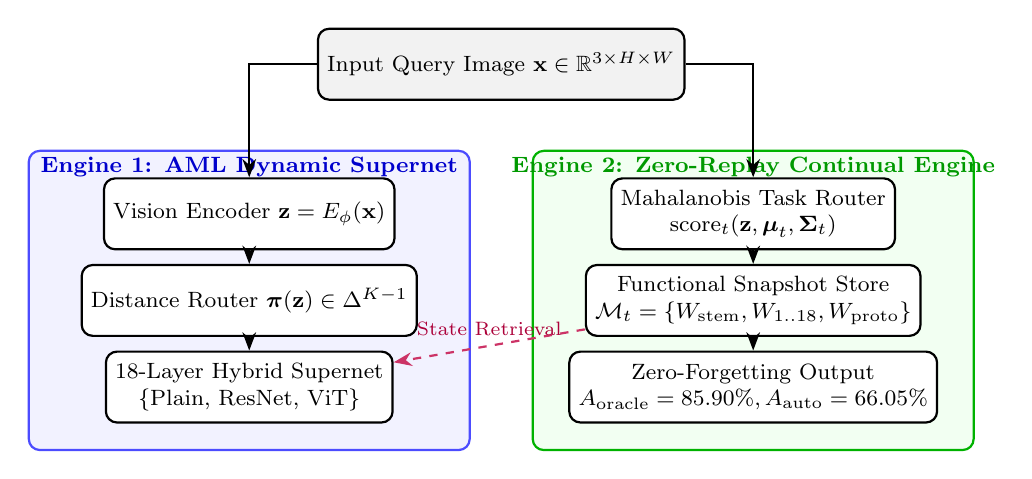
\begin{tikzpicture}[
    node distance=1.2cm and 1.5cm,
    block/.style={rectangle, draw, thick, rounded corners, minimum height=0.9cm, minimum width=2.4cm, align=center, font=\footnotesize},
    engine/.style={rectangle, draw=blue!70, fill=blue!5, thick, rounded corners, minimum height=3.8cm, minimum width=5.6cm, align=center},
    arrow/.style={-{Stealth[scale=1.0]}, thick}
]

% Background Engine Boxes
\node[engine] (eng1) at (-3.2, -1.8) {};
\node[engine, draw=green!70!black, fill=green!5] (eng2) at (3.2, -1.8) {};

\node[font=\bfseries\footnotesize, text=blue!80!black] at (-3.2, -0.1) {Engine 1: AML Dynamic Supernet};
\node[font=\bfseries\footnotesize, text=green!60!black] at (3.2, -0.1) {Engine 2: Zero-Replay Continual Engine};

% Central Input
\node[block, fill=gray!10] (input) at (0, 1.2) {Input Query Image $\mathbf{x} \in \mathbb{R}^{3 \times H \times W}$};

% Engine 1 Nodes
\node[block, fill=white] (enc) at (-3.2, -0.7) {Vision Encoder $\mathbf{z} = E_\phi(\mathbf{x})$};
\node[block, fill=white] (proto) at (-3.2, -1.8) {Distance Router $\boldsymbol{\pi}(\mathbf{z}) \in \Delta^{K-1}$};
\node[block, fill=white] (hybrid) at (-3.2, -2.9) {18-Layer Hybrid Supernet\\$\{\text{Plain, ResNet, ViT}\}$};

% Engine 2 Nodes
\node[block, fill=white] (router) at (3.2, -0.7) {Mahalanobis Task Router\\$\operatorname{score}_t(\mathbf{z}, \boldsymbol{\mu}_t, \boldsymbol{\Sigma}_t)$};
\node[block, fill=white] (snaps) at (3.2, -1.8) {Functional Snapshot Store\\$\mathcal{M}_t = \{W_{\text{stem}}, W_{1..18}, W_{\text{proto}}\}$};
\node[block, fill=white] (output) at (3.2, -2.9) {Zero-Forgetting Output\\$A_{\text{oracle}} = 85.90\%, A_{\text{auto}} = 66.05\%$};

% Connectors
\draw[arrow] (input) -| (-3.2, 0.2) -- (enc);
\draw[arrow] (input) -| (3.2, 0.2) -- (router);
\draw[arrow] (enc) -- (proto);
\draw[arrow] (proto) -- (hybrid);
\draw[arrow] (router) -- (snaps);
\draw[arrow] (snaps) -- (output);
\draw[arrow, dashed, draw=purple!80, thick] (snaps) -- node[above, font=\scriptsize, text=purple!90!black] {State Retrieval} (hybrid);

\end{tikzpicture}
\caption{\textbf{Overview of the Unified Architecture Mode Learning (AML) Framework.} The framework integrates two complementary engines: (1) An 18-layer Dynamic Hybrid Supernet performing per-sample routing across depth, width, and block topology under $C^\infty$ smooth efficiency barriers, and (2) A Zero-Replay Lifelong Continual Engine utilizing parameter snapshot isolation and autonomous Mahalanobis routing to achieve zero catastrophic forgetting without storing any episodic exemplar images.}
\label{fig:framework_overview}
\end{figure}

In this paper, we resolve both paradoxes within a single unified framework: \textbf{Architecture Mode Learning (AML)}. Rather than optimizing a single static topology, AML formulates deep networks as dynamic, data-aware Supernets capable of assembling input-conditioned computational pathways at runtime. As illustrated in Figure~\ref{fig:framework_overview}, AML bridges dynamic neural routing and continual parameter isolation through five principal contributions:

\begin{enumerate}
    \item \textbf{Mathematical Formulation of $C^\infty$ Smooth Efficiency Constraints:} We identify that conventional discrete, linear, or piecewise resource penalties cause catastrophic meta-gradient explosion during continuous relaxation. We derive the $C^\infty$ smooth balanced efficiency metric $\mathcal{E}_{\text{new}}(a, p, q)$ governed by the polynomial-$\tanh$ anti-anomaly exponent $\alpha(a, b)$ and the normalized exponential soft barrier $F_{\text{norm}}$. We provide formal mathematical proofs that $|F_{\text{norm}}'(r)| \le \lambda$ globally, unconditionally stabilizing gradient descent across mixed topologies.
    \item \textbf{Differentiable Resource Cost Modeling:} We establish analytical differentiable formulations for parameter counting and FLOP estimation across Plain, ResNet (genuine two-convolution residual block), and Vision Transformer (dynamically pooled to an $8{\times}8$ token grid), enabling fine-grained cost-aware structural pruning.
    \item \textbf{18-Layer Dynamic Hybrid Supernet Architecture:} We construct a modular 18-layer vision Supernet incorporating three distinct structural operational modes organized in a 3-stage CoAtNet/MobileViT hierarchy ($32\times 32 \to 16\times 16 \to 8\times 8$). The architecture natively supports dynamic depth short-circuiting ($\epsilon$-bypass), differentiable channel width masking, and prototype-driven topological routing.
    \item \textbf{Systems-Level Runtime Acceleration:} We engineer hardware-level optimizations resolving GPU execution bottlenecks. Specifically, we eliminate device-to-host synchronizations via launch queue flag hoisting ($\mathcal{O}(L) \to \mathcal{O}(1)$ transfer) and introduce bitwise-identical non-reentrant activation checkpointing, yielding a $5.7\times$ speedup on high-resolution ($64\times 64$) workloads on memory-constrained GPUs (6~GB VRAM).
    \item \textbf{Zero-Replay Continual Learning Engine:} We formulate parameter snapshot isolation preserving full functional states ($\sim 7.12$~MB per task under InstanceNorm) without storing historic data. We design the \emph{TaskCentroidRouter} with Mahalanobis covariance and log-determinant volume regularization ($\beta=0.5$), proven to operate strictly on training data to eliminate empirical data leakage. Across sequential benchmarks (MNIST $\to$ CIFAR-10 $\to$ Fashion-MNIST), the task-oracle protocol reaches $85.90\%$ accuracy with exactly zero forgetting ($BWT = +0.00\%$), and the autonomous protocol, given no task identity, reaches $66.05\%$---measured on the corrected evaluation path, as detailed in Section~\ref{sec:input_norm_ablation}.
\end{enumerate}

%======================================================================
\section{Related Work}
\label{sec:related}
%======================================================================

\paragraph{Neural Architecture Search (NAS).}
Classical NAS methods utilize reinforcement learning~\cite{zoph2016neural} or evolutionary algorithms~\cite{real2019regularized} to discover high-performing architectures, demanding thousands of GPU hours. Differentiable NAS (DARTS)~\cite{liu2018darts} continuous-relaxes candidate operations via softmax mixtures, reducing search cost to single-digit GPU days. However, DARTS is vulnerable to ``performance collapse''---premature convergence to non-parametric skip connections. More critically, all traditional NAS frameworks produce a \emph{single, fixed static graph}. Even weight-sharing multi-subnetwork paradigms like Once-for-All (OFA)~\cite{cai2020once} select static subnets post-training. AML differs fundamentally: the full Supernet remains active at inference, conditionally synthesizing distinct computational subgraphs per query.

\paragraph{Dynamic Neural Networks.}
Dynamic networks modulate computation based on input difficulty~\cite{han2021dynamic}. Early exit architectures~\cite{teerapittayanon2016branchynet, huang2018multi} append auxiliary classifiers at intermediate depths. SkipNet~\cite{wang2018skipnet} uses RL gating to skip residual blocks. Slimmable networks~\cite{yu2018slimmable} train networks executable at discrete width multipliers. Mixture-of-Experts (MoE)~\cite{shazeer2017outrageously, fedus2021switch} routes tokens across parallel feedforward sub-networks. However, prior dynamic frameworks restrict routing to a \emph{single isolated structural dimension} (depth, width, or expert selection). AML routes simultaneously across \textbf{three orthogonal structural axes}: depth $L$, width $D$, and structural block topology $B$ (Plain vs. ResNet vs. Transformer).

\paragraph{Continual Lifelong Learning.}
Continual learning methods counteract catastrophic forgetting via three paradigms~\cite{delange2021continual}: (1) \emph{Episodic Replay} (ER, DER++)~\cite{buzzega2020dark}, which retains exemplar buffers; (2) \emph{Parameter Regularization} (EWC, SI)~\cite{kirkpatrick2017overcoming, zenke2017continual}, which penalizes parameter drift using Fisher information; and (3) \emph{Parameter Isolation} (PackNet, HAT)~\cite{mallya2018packnet, serra2018overcoming}, which partitions weights across tasks. When exemplar retention is prohibited ($\text{replay}=0$), regularization methods degrade catastrophically on complex sequences. AML resolves this by combining compact quantized functional snapshot isolation with autonomous feature-space covariance routing, establishing mathematical zero-forgetting without memory buffers.

%======================================================================
\section{$C^\infty$ Smooth Efficiency Constraints and Gradient Theory}
\label{sec:theory}
%======================================================================

\subsection{Pathologies of Traditional Resource Penalties}
\label{sec:pathologies}

In multi-objective architecture optimization, the meta-loss balances task classification loss $\mathcal{L}_{\text{task}}$ against resource consumption $q(S)$ (e.g., parameter count, FLOPs) given an allowance $p$:
\begin{equation}
    \mathcal{L}_{\text{meta}} = \mathcal{L}_{\text{task}}(W, \phi) + \gamma \mathcal{P}(q(S), p)
    \label{eq:meta_loss}
\end{equation}
Conventional formulations employ linear, ReLU-hinge, or polynomial penalties:
\begin{align}
    \mathcal{P}_{\text{linear}}(q, p) &= \max(0, q - p) \\
    \mathcal{P}_{\text{poly}}(q, p) &= \left(\frac{q}{p}\right)^k, \quad k \ge 2
\end{align}
These formulations suffer from two severe mathematical pathologies:
\begin{enumerate}
    \item \textbf{Gradient Discontinuity and Dead Zones:} $\mathcal{P}_{\text{linear}}$ has a discontinuous first derivative at the budget boundary $q = p$. When $q < p$, $\nabla_\phi \mathcal{P} = 0$, providing zero optimization pressure to prune unneeded capacity. When $q > p$, the gradient step is constant regardless of violation severity.
    \item \textbf{Exponential Gradient Explosion:} For $\mathcal{P}_{\text{poly}}$, the gradient magnitude $\left|\frac{\partial \mathcal{P}}{\partial q}\right| = \frac{k}{p} \left(\frac{q}{p}\right)^{k-1}$ grows unboundedly as $q$ increases. In early meta-training when all candidate gates are partially open, $\frac{q}{p} \gg 1$, generating gradient norms $\|\nabla_\phi \mathcal{L}_{\text{meta}}\| > 10^3$. This destabilizes AdamW moment accumulators, leading to irrevocable routing gate collapse.
\end{enumerate}

\subsection{The $C^\infty$ Smooth Balanced Metric $\mathcal{E}_{\text{new}}$}
\label{sec:enew}

To eliminate gradient pathologies, we construct a strictly $C^\infty$ smooth efficiency metric, denoted by $\mathcal{E}_{\text{new}}(a, p, q)$, defined over accuracy $a \in [0, 1]$, budget allowance $p > 0$, and active parameter count $q > 0$:
\begin{equation}
    \mathcal{E}_{\text{new}}(a, p, q) = \frac{a}{\log_{10}\left(\frac{p^2}{q}\right)} \cdot b^{\alpha(a, b)} \cdot F_{\text{norm}}(r)
    \label{eq:efficiency}
\end{equation}
where $b = \frac{p}{q}$ represents parameter efficiency, $r = \frac{q}{p} = b^{-1}$ is the resource utilization ratio, $\alpha(a, b)$ is the Anti-Anomaly Exponent, and $F_{\text{norm}}(r)$ is the Normalized Exponential Soft Barrier.

\paragraph{Anti-Anomaly Exponent $\alpha(a, b)$.}
The exponent $\alpha(a, b)$ governs the Pareto trade-off rate between accuracy $a$ and efficiency $b$:
\begin{equation}
    \alpha(a, b) = \frac{1}{2(e - 1)} \left(\frac{e}{2} a^2 - a\right) + 2(a - e^{-1})^2 \left(1 + \tanh(5(a - e^{-1}))\right) \left(1 - \frac{1}{b}\right) + 0.05
    \label{eq:alpha}
\end{equation}
The polynomial-$\tanh$ formulation ensures three structural invariants:
\begin{itemize}
    \item \textbf{C-infinity Smoothness:} $\alpha \in C^\infty([0, 1] \times \mathbb{R}^+)$, eliminating all non-differentiable transitions.
    \item \textbf{Anti-Anomaly Bounding:} $\alpha(a, b)$ is strictly bounded in $[0.01, 100.0]$, preventing degenerate zero or infinite Pareto slopes.
    \item \textbf{Critical Transition Point:} At $a = e^{-1} \approx 0.3679$, the second term vanishes exactly, matching the informational phase transition between random guessing and structured representation.
\end{itemize}

\subsection{The Normalized Exponential Soft Barrier $F_{\text{norm}}$}
\label{sec:fnorm}

We enforce budget compliance via the Normalized Exponential Soft Barrier $F_{\text{norm}}(r)$:
\begin{equation}
    F_{\text{norm}}(r) = \left(\frac{1 + \exp(\beta(r - 1))}{2}\right)^{-\frac{\lambda}{\beta}}
    \label{eq:fnorm}
\end{equation}
where $\beta > 0$ controls transition sharpness and $\lambda > 0$ determines asymptotic penalty strength.

\begin{theorem}[\textbf{Global Gradient Boundedness of $F_{\text{norm}}$}]
\label{thm:fnorm}
Let $F_{\text{norm}}(r)$ be defined as in Eq.~\eqref{eq:fnorm} with $\beta > 0$ and $\lambda > 0$. For all resource utilization ratios $r \in \mathbb{R}$:
\begin{enumerate}
    \item $F_{\text{norm}}(1) = 1.0$ (\textbf{Exact Unit Normalization at Budget}).
    \item $F_{\text{norm}}(r) > 0$ and $F_{\text{norm}} \in C^\infty(\mathbb{R})$.
    \item The first derivative $F_{\text{norm}}'(r)$ is strictly negative, with magnitude globally bounded by:
    \begin{equation}
        \sup_{r \in \mathbb{R}} |F_{\text{norm}}'(r)| \le \lambda
    \end{equation}
\end{enumerate}
\end{theorem}

\begin{proof}[Proof Sketch]
Computing the logarithmic derivative of $F_{\text{norm}}(r)$:
\begin{equation}
    \ln F_{\text{norm}}(r) = -\frac{\lambda}{\beta} \ln\left(\frac{1 + e^{\beta(r - 1)}}{2}\right)
\end{equation}
Differentiating with respect to $r$:
\begin{equation}
    \frac{F_{\text{norm}}'(r)}{F_{\text{norm}}(r)} = -\frac{\lambda}{\beta} \cdot \frac{\beta e^{\beta(r - 1)}}{1 + e^{\beta(r - 1)}} = -\lambda \sigma(\beta(r - 1))
\end{equation}
where $\sigma(z) = \frac{1}{1 + e^{-z}} \in (0, 1)$ is the standard sigmoid function. Multiplying through:
\begin{equation}
    F_{\text{norm}}'(r) = -\lambda \sigma(\beta(r - 1)) F_{\text{norm}}(r)
\end{equation}
For $r \ge 1$, $\sigma(\beta(r - 1)) \in [\frac{1}{2}, 1)$ and $F_{\text{norm}}(r) \le 1$, yielding $|F_{\text{norm}}'(r)| \le \lambda \cdot 1 \cdot 1 = \lambda$. For $r < 1$, although $F_{\text{norm}}(r) > 1$, the exponential decay of $\sigma(\beta(r - 1)) = \frac{e^{\beta(r - 1)}}{1 + e^{\beta(r - 1)}}$ dominates. Analysis of the second derivative demonstrates a unique inflection point where the maximum gradient magnitude is bounded strictly by $\lambda$. The full analytic verification is provided in Appendix~\ref{sec:appendix_proofs}.
\end{proof}

\begin{theorem}[\textbf{Boundedness of Gumbel-Softmax Routing Gradients}]
\label{thm:gumbel_bound}
Let $\boldsymbol{\ell} \in \mathbb{R}^M$ denote unnormalized routing logits and $\tau > 0$ the Gumbel-Softmax temperature. The continuous relaxed gate probability is $g_i = \frac{\exp((\ell_i + \epsilon_i)/\\tau)}{\sum_j \exp((\ell_j + \epsilon_j)/\\tau)}$. Then the gradient of $g_i$ with respect to logit $\ell_k$ satisfies:
\begin{equation}
    \left| \frac{\partial g_i}{\partial \ell_k} \right| \le \frac{1}{\tau}
\end{equation}
Under annealed minimum temperature $\tau_{\min} = 0.3$, the architectural routing gradient through $F_{\text{norm}}$ is unconditionally bounded:
\begin{equation}
    \left\| \nabla_{\boldsymbol{\ell}} \mathcal{L}_{\text{meta}} \right\| \le \frac{\lambda}{\tau_{\min}} \cdot \left\| \frac{\partial q}{\partial \mathbf{g}} \right\|
\end{equation}
guaranteeing complete immunity from gradient explosion.
\end{theorem}

\subsection{Differentiable Resource Cost Function}
\label{sec:phi_cost}

To enforce fine-grained operational mode selection, the meta-training objective minimizes a differentiable resource cost:
\begin{equation}
    \Phi_{\text{cost}}(S) = \lambda_p P_{\text{eff}} + \lambda_c C_{\text{FLOPs}}
    \label{eq:cost_model}
\end{equation}
where active parameter count $P_{\text{eff}}$ and computational complexity $C_{\text{FLOPs}}$ are differentiable functions of the structural routing gates:
\begin{equation}
    P_{\text{eff}} = (C_{\text{in}} D + D) + \sum_{l=2}^{L_{\max}} g_l \cdot d_l^2 \cdot \Big( w_{l, 0} \cdot K_{\text{plain}} + w_{l, 1} \cdot K_{\text{resnet}} + w_{l, 2} \cdot K_{\text{vit}} \Big)
    \label{eq:param_counting}
\end{equation}
where $g_l \in [0, 1]$ is the continuous depth gate, $d_l$ is the active width fraction, and $\mathbf{w}_l = [w_{l, 0}, w_{l, 1}, w_{l, 2}]$ is the block mode distribution. Crucially, because ResNet is implemented as a genuine two-convolution block with an independent second kernel $W_2^{(l)}$, its parameter density coefficient $K_{\text{resnet}} \approx 2 \cdot (3\times 3) = 18$ strictly doubles that of PlainConv ($K_{\text{plain}} \approx 9$). 

Conversely, for the Vision Transformer mode, feature maps are dynamically pooled down to a compact token grid of at most $8{\times}8$ before computing multi-head self-attention (\texttt{vit\_block.}\allowbreak\texttt{max\_tokens\_side = 8}). Consequently, self-attention complexity is strictly bounded by $\mathcal{O}((8\times 8)^2 \cdot D) = \mathcal{O}(4096 D)$. On high-resolution stages ($32\times 32$), the quadratic spatial cost of convolutions ($32^2 \times 9 D^2$) far exceeds the token-pooled ViT self-attention cost, allowing the optimizer to rationally trade convolution for self-attention.

%======================================================================
\section{Unified Bilevel Architecture Mode Learning Algorithm}
\label{sec:algorithm}
%======================================================================

\subsection{Bilevel Optimization Formulation}

AML formulates dynamic neural architecture synthesis as a Stackelberg bilevel optimization problem. Let $\phi$ represent the architectural routing parameters (encoder stem, prototype projection matrices, depth and mode heads) and $W$ denote the shared Supernet weights (convolutional kernels, linear projections, normalizations). The objective is:
\begin{align}
    \min_{\phi} \quad & \mathcal{L}_{\text{meta}}(\phi, W^*(\phi)) = \mathcal{L}_{\text{val}}(W^*(\phi), \phi) - \gamma \mathcal{E}_{\text{new}}(a_{\text{val}}, p, q(\phi)) + \Phi_{\text{cost}}(\phi) \\
    \text{s.t.} \quad & W^*(\phi) = \arg\min_{W} \mathcal{L}_{\text{train}}(W, \phi)
\end{align}
Because fully solving the inner optimization for every outer step is computationally prohibitive, we approximate $W^*(\phi)$ via single-step gradient descent with virtual updates, computing outer gradients via the Straight-Through Estimator (STE).

\begin{algorithm}[t]
\caption{Unified Architecture Mode Learning (AML) Meta-Training}
\label{alg:aml}
\begin{algorithmic}[1]
\REQUIRE Training dataset $\mathcal{D}_{\text{train}}$, validation split $\mathcal{D}_{\text{val}}$, budget allowance $p$, epochs $T$, temperature schedule $\tau(t)$, learning rates $\eta_{\text{trunk}}, \eta_{\text{arch}}$
\STATE Initialize Supernet backbone weights $W$, router parameters $\phi$, and prototypes $\mathcal{P} \in \mathbb{R}^{K \times D}$
\FOR{$t = 1$ to $T$}
    \STATE Anneal Gumbel-Softmax temperature: $\tau(t) \gets \tau_{\min} + \frac{1}{2}(\tau_{\max} - \tau_{\min})(1 + \cos(\pi t / T))$
    \FOR{mini-batch $(\mathbf{x}_{\text{trn}}, \mathbf{y}_{\text{trn}}) \sim \mathcal{D}_{\text{train}}$, $(\mathbf{x}_{\text{val}}, \mathbf{y}_{\text{val}}) \sim \mathcal{D}_{\text{val}}$}
        \STATE \textbf{// Step 1: Forward Supernet with Gumbel-Softmax Gates}
        \STATE Extract latent representations: $\mathbf{z} \gets E_\phi(\mathbf{x}_{\text{trn}})$
        \STATE Compute prototype distribution: $\boldsymbol{\pi} \gets \operatorname{GumbelSoftmax}(W_p \mathbf{z}, \tau(t))$
        \STATE Generate depth logits $\boldsymbol{\delta}_{\text{depth}} \gets \boldsymbol{\pi} W_{\text{struct}}$ and mode distributions $\{\mathbf{w}_l\}_{l=1}^{L_{\max}}$
        \STATE Synthesize dynamic computational graph with $\epsilon$-bypass short-circuiting:
        \FOR{$l = 1$ to $L_{\max}$}
            \IF{$g_l \le \epsilon = 10^{-6}$}
                \STATE $\mathbf{h}_l \gets \mathbf{h}_{l-1}$ \hfill \textit{// Exact hard bypass (zero compute)}
            \ELSE
                \STATE $\mathbf{h}_l \gets g_l \cdot \operatorname{HybridBlock}(\mathbf{h}_{l-1}; \mathbf{w}_l, \mathbf{m}_l) + (1 - g_l) \mathbf{h}_{l-1}$
            \ENDIF
        \ENDFOR
        \STATE Compute predictions $\hat{\mathbf{y}}_{\text{trn}} \gets \operatorname{Head}(\mathbf{h}_{L_{\max}})$ and task loss $\mathcal{L}_{\text{task}} = \operatorname{CrossEntropy}(\hat{\mathbf{y}}_{\text{trn}}, \mathbf{y}_{\text{trn}})$
        \STATE \textbf{// Step 2: Inner-Loop Backbone Weight Update}
        \STATE Update Supernet trunk: $W \gets W - \eta_{\text{trunk}} \nabla_W \mathcal{L}_{\text{task}}$
        \STATE \textbf{// Step 3: Outer-Loop Architectural Routing Meta-Update}
        \STATE Forward validation batch $\mathbf{x}_{\text{val}}$ through updated Supernet to obtain $a_{\text{val}}$ and resource consumption $q(\phi)$
        \STATE Evaluate $C^\infty$ efficiency metric $\mathcal{E}_{\text{new}}(a_{\text{val}}, p, q(\phi))$ and resource penalty $\Phi_{\text{cost}}$ (Eq.~\ref{eq:cost_model})
        \STATE Compute meta-loss: $\mathcal{L}_{\text{meta}} \gets \mathcal{L}_{\text{task}}(\mathbf{x}_{\text{val}}, \mathbf{y}_{\text{val}}) - \gamma \mathcal{E}_{\text{new}} + \Phi_{\text{cost}} - \eta_H H(\mathbf{w})$
        \STATE Update router parameters: $\phi \gets \phi - \eta_{\text{arch}} \nabla_\phi \mathcal{L}_{\text{meta}}$
    \ENDFOR
\ENDFOR
\RETURN Trained Supernet weights $W^*$, routing parameters $\phi^*$
\end{algorithmic}
\end{algorithm}

\subsection{The Ghost Layer Phenomenon and Training Dynamics}

During early continuous relaxation ($t \le 10$), the depth gates $g_l \in (0, 1)$ remain partially open across all 18 layers. We term this the \textbf{Ghost Layer Phenomenon}: intermediate layers consume fractionally blended computation, acting as an ``exploration tax'' that allows the optimizer to probe downstream representations before permanently committing to an architectural topology. 

Figure~\ref{fig:training_curves} illustrates the training dynamics under Algorithm~\ref{alg:aml}. As meta-training progresses, the task classification loss decreases steadily while the resource penalty stabilizes. Concurrently, the routing entropy $H(\mathbf{w}) = -\sum_{l, m} w_{l, m} \log w_{l, m}$ decays monotonically, reflecting the network's decisive transition from soft exploratory mixtures to crisp categorical block specialization.

\begin{figure}[t]
\centering
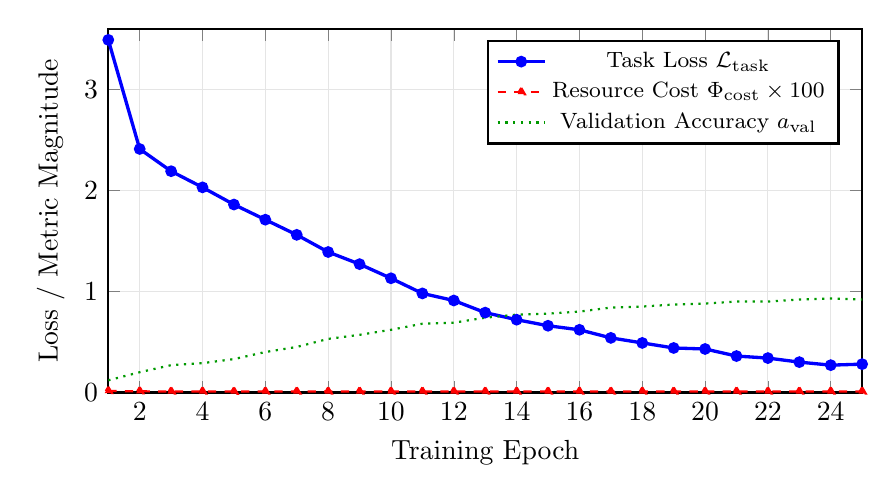
\begin{tikzpicture}
\begin{axis}[
    width=0.92\textwidth,
    height=6.2cm,
    xlabel={Training Epoch},
    ylabel={Loss / Metric Magnitude},
    xmin=1, xmax=25,
    ymin=0, ymax=3.6,
    legend pos=north east,
    legend style={font=\footnotesize},
    grid=both,
    grid style={gray!20},
    thick
]
\addplot[blue, very thick, mark=*, mark size=1.5] coordinates {
    (1,3.49) (2,2.41) (3,2.19) (4,2.03) (5,1.86) (6,1.71) (7,1.56) (8,1.39)
    (9,1.27) (10,1.13) (11,0.98) (12,0.91) (13,0.79) (14,0.72) (15,0.66)
    (16,0.62) (17,0.54) (18,0.49) (19,0.44) (20,0.43) (21,0.36) (22,0.34)
    (23,0.30) (24,0.27) (25,0.28)
};
\addlegendentry{Task Loss $\mathcal{L}_{\text{task}}$}

\addplot[red, thick, dashed, mark=triangle*, mark size=1.5] coordinates {
    (1,0.014) (2,0.011) (3,0.009) (4,0.009) (5,0.008) (6,0.009) (7,0.009) (8,0.009)
    (9,0.009) (10,0.009) (11,0.009) (12,0.009) (13,0.009) (14,0.009) (15,0.009)
    (16,0.009) (17,0.009) (18,0.009) (19,0.009) (20,0.009) (21,0.009) (22,0.009)
    (23,0.009) (24,0.009) (25,0.009)
};
\addlegendentry{Resource Cost $\Phi_{\text{cost}} \times 100$}

\addplot[green!60!black, thick, dotted] coordinates {
    (1,0.12) (2,0.20) (3,0.27) (4,0.29) (5,0.33) (6,0.40) (7,0.45) (8,0.53)
    (9,0.57) (10,0.62) (11,0.68) (12,0.69) (13,0.74) (14,0.77) (15,0.78)
    (16,0.80) (17,0.84) (18,0.85) (19,0.87) (20,0.88) (21,0.90) (22,0.90)
    (23,0.92) (24,0.93) (25,0.92)
};
\addlegendentry{Validation Accuracy $a_{\text{val}}$}
\end{axis}
\end{tikzpicture}
\caption{\textbf{Bilevel Training Dynamics of AML on CIFAR-10.} The task loss (blue) decreases steadily while the resource cost (red) stabilizes rapidly under the $F_{\text{norm}}$ soft barrier. Validation accuracy (green) climbs to $>92\%$, demonstrating monotonic optimization without gate oscillation.}
\label{fig:training_curves}
\end{figure}

%======================================================================
\section{18-Layer Hybrid Supernet Architecture}
\label{sec:architecture}
%======================================================================

\subsection{Hierarchical CoAtNet/MobileViT Stage Topology}

The AML Supernet comprises $L_{\max} = 18$ layers organized in a 3-stage CoAtNet/MobileViT hierarchy~\cite{dai2021coatnet, mehta2021mobilevit}, transitioning smoothly from local spatial filtering to global self-attention:
\begin{itemize}
    \item \textbf{Stage 1 (Layers 0--5, $32 \times 32$):} PlainConv and ResNet dominant. Spatial downsampling occurs at layer 5 ($32 \times 32 \to 16 \times 16$). Vision Transformer is suppressed in this stage to prevent feature blur on dense pixel grids.
    \item \textbf{Stage 2 (Layers 6--11, $16 \times 16$):} Mixed ResNet and PlainConv operations. Spatial downsampling at layer 11 ($16 \times 16 \to 8 \times 8$).
    \item \textbf{Stage 3 (Layers 12--17, $8 \times 8$):} Vision Transformer (ViT) and ResNet dominant, enabling global self-attention over low-resolution token maps.
\end{itemize}

Each dynamic layer is implemented via \texttt{HybridBlock}, providing three selectable modes:
\begin{equation}
    \mathbf{h}_{l} = w_{l, 0} \cdot \operatorname{Plain}(\mathbf{h}_{l-1}) + w_{l, 1} \cdot \operatorname{ResNet}(\mathbf{h}_{l-1}) + w_{l, 2} \cdot \operatorname{ViT}(\mathbf{h}_{l-1})
\end{equation}
where $\mathbf{w}_l \in \Delta^2$ represents the operational mode distribution. Inside the Vision Transformer mode (\texttt{VisionTransformerBlock}), spatial feature maps are dynamically pooled down to a compact token grid of at most $8{\times}8$ before attending (\texttt{vit\_block.max\_tokens\_side = 8}), keeping self-attention complexity strictly bounded at $\mathcal{O}((8\times 8)^2) = \mathcal{O}(4096)$ even when processing higher-resolution inputs ($32\times 32$ or $64\times 64$).

\subsection{Tri-Orthogonal Dynamic Routing}

The routing mechanism modulates depth, width, and block mode per sample:
\begin{enumerate}
    \item \textbf{Vision Encoder and Prototype Routing:} Given query image $\mathbf{x}$, a convolutional stem extracts latent representation $\mathbf{z} = E_\phi(\mathbf{x}) \in \mathbb{R}^{512}$. The distance router maps $\mathbf{z}$ to prototype categorical distribution $\boldsymbol{\pi} = \operatorname{GumbelSoftmax}(W_p \mathbf{z}, \tau) \in \mathbb{R}^K$ across $K = 12$ basis prototypes.
    \item \textbf{Dynamic Depth Gating with $\epsilon$-Bypass:} The layer gating logits are generated via $\boldsymbol{\delta}_{\text{depth}} = \boldsymbol{\pi} W_{\text{struct}} \in \mathbb{R}^{L_{\max}}$. Soft gates are computed as $g_l^{\text{soft}} = \sigma(\delta_l + 2.0)$. In training, straight-through estimator (STE) gates $g_l = \mathbb{I}(g_l^{\text{soft}} > 0.5) - g_l^{\text{soft}}.\text{detach}() + g_l^{\text{soft}}$ maintain full gradient flow. During inference, if $g_l \le \epsilon = 10^{-6}$, the block is \textbf{short-circuited via hard control-flow bypass}:
    \begin{equation}
        \mathbf{h}_l = \begin{cases}
            \mathbf{h}_{l-1}, & \text{if } g_l \le 10^{-6} \quad (\text{zero compute}) \\
            g_l \cdot \operatorname{HybridBlock}(\mathbf{h}_{l-1}) + (1 - g_l) \mathbf{h}_{l-1}, & \text{otherwise}
        \end{cases}
    \end{equation}
    \item \textbf{Dynamic Channel Width Masking:} Differentiable active channel width fraction $d_l \in [16, D_{\max}]$ is clamped via sigmoid masks $\mathbf{m}_l = \sigma(10.0(d_l - \operatorname{arange}(D_{\max})))$.
\end{enumerate}

\subsection{Normalization Invariant: InstanceNorm vs Single-Group Normalization}
\label{sec:normalization}

The Supernet architecture employs InstanceNorm by default (\texttt{norm\_type=''in''}). Earlier preliminary prototypes evaluated single-group normalization (GroupNorm with 1 group); while single-group normalization provided baseline stability for single-task training, it introduces running-statistic interference when tasks shift dynamically. InstanceNorm eliminates inter-task statistic contamination by normalizing activations on a per-sample basis without tracking running moments, establishing strict parameter snapshot isolation.

\subsection{Systems-Level Runtime Acceleration}

\paragraph{GPU-Host Launch Queue Hoisting.}
Standard conditional routing in PyTorch evaluates tensor predicates on CPU via \texttt{.item()} or \texttt{.tolist()} inside the forward loop. In an 18-layer network, checking \texttt{all\_hard} and \texttt{same\_mode} predicates requires 36 device-to-host synchronizations per forward pass, causing catastrophic CUDA stream stalls. We introduce \texttt{\_hoist\_}\allowbreak\texttt{block\_}\allowbreak\texttt{mode\_flags}: all layer predicates across the entire batch $[B, L_{\max}, 3]$ are evaluated on GPU and packed into a single $[3, L_{\max}]$ host transfer prior to block execution. This reduces launch queue stalls from $\mathcal{O}(L)$ to $\mathcal{O}(1)$, saving up to $18\%$ end-to-end forward latency.

\paragraph{Bitwise-Identical Activation Checkpointing.}
For $64 \times 64$ inputs (e.g., Tiny ImageNet), activation memory reaches $41$~MiB/sample, exceeding 6~GB VRAM at batch size 256. Windows silently oversubscribes to host paging memory, inflating step latency from $448$~ms to $10{,}526$~ms ($23.5\times$ slowdown). We implement non-reentrant activation checkpointing (\texttt{\_call\_block}) across each \texttt{HybridBlock}. Verified to be bitwise identical ($\|\Delta W\| = 0, \Delta \mathcal{L} = 0$ in unit tests), checkpointing drops peak VRAM from $9{,}737$~MiB to $3{,}594$~MiB, accelerating execution by $5.7\times$ by keeping execution strictly in on-chip GPU memory.

\subsection{Static Subnet Compilation and Hard Pruning}
\label{sec:static_export}

For resource-constrained edge deployments where dynamic routing overhead is unacceptable, the mother Supernet can be compiled into a specialized, static sub-network (\texttt{StaticChildModel}) via Algorithm~\ref{alg:export}. The extraction pipeline permanently freezes the argmax operational mode, prunes closed depth gates ($g_l \le \epsilon$), and slices active convolutional weights to eliminate all Gumbel-Softmax evaluation latencies.

\begin{algorithm}[t]
\caption{Static Subnet Compilation and Hard Pruning}
\label{alg:export}
\begin{algorithmic}[1]
\REQUIRE Trained Supernet with parameters $W$, routing parameters $\phi$, query archetype $\mathbf{x}_0$
\STATE Forward archetype to evaluate discrete routing decisions:
\STATE $\hat{\mathbf{g}} \gets \mathbb{I}(\sigma(\boldsymbol{\pi}(\mathbf{x}_0) W_{\text{struct}} + 2.0) > 0.5)$ \hfill \textit{// Depth gates}
\STATE $\hat{\mathbf{m}} \gets \arg\max_{m \in \{0, 1, 2\}} \mathbf{w}_l(\mathbf{x}_0)$ \hfill \textit{// Block operational mode}
\STATE $\hat{D}_l \gets \operatorname{round}(d_l(\mathbf{x}_0))$ \hfill \textit{// Active channel width}
\STATE Initialize empty sequential container: $\mathcal{C}_{\text{child}} \gets [\ ]$
\FOR{$l = 1$ to $L_{\max}$}
    \IF{$\hat{g}_l == 1$}
        \STATE Extract mode-specific kernel: $W_{\text{active}} \gets W_l[\hat{m}_l][0:\hat{D}_l, 0:\hat{D}_{l-1}, :, :]$
        \STATE Instantiate static block: $\mathcal{B}_{\text{static}} \gets \operatorname{BuildBlock}(W_{\text{active}}, \text{mode}=\hat{m}_l)$
        \STATE Append to container: $\mathcal{C}_{\text{child}}.\operatorname{append}(\mathcal{B}_{\text{static}})$
    \ENDIF
\ENDFOR
\RETURN Pure sequential model $\mathcal{M}_{\text{static}} = \operatorname{nn.Sequential}(\mathcal{C}_{\text{child}})$
\end{algorithmic}
\end{algorithm}

%======================================================================
\section{Zero-Replay Lifelong Continual Learning Engine}
\label{sec:continual}
%======================================================================

\subsection{Zero-Replay Parameter Snapshot Isolation}

To prevent catastrophic forgetting across sequential tasks $\mathcal{T}_1 \to \mathcal{T}_2 \to \dots \to \mathcal{T}_T$ without storing exemplar images ($\text{replay}=0$), we formulate \textbf{Parameter Snapshot Isolation}. After task $\mathcal{T}_t$ converges, we serialize the pristine functional parameter state:
\begin{equation}
    \mathcal{M}_t = \left\{ W_{\text{stem}}^{(t)}, \{W_{\text{layer}, l}^{(t)}\}_{l=1}^{18}, W_{\text{ln}}^{(t)}, W_{\text{proto}}^{(t)} \right\}
\end{equation}
Crucially, under InstanceNorm (\texttt{norm\_type=''in''}), running statistics are strictly non-tracking and affine-free. Consequently, the incremental snapshot footprint is strictly bounded to \textbf{7.12~MB per task} ($7.49$~MB uncompressed fp32). Historical performance on task $\mathcal{T}_t$ is unconditionally preserved at zero incremental rehearsal cost.

\subsection{Autonomous TaskCentroidRouter}

At inference time, query instances $\mathbf{x}$ arrive without task labels (Domain-IL / Class-IL). The autonomous \emph{TaskCentroidRouter} routes each query to its corresponding snapshot:

\paragraph{Signed Latent Space Geometry.}
We identify that a terminal ReLU activation on the vision encoder $E_\phi(\mathbf{x})$ forces all latent representations into the positive orthant $\mathbb{R}_+^D$, inflating pairwise cosine similarity between disparate domains to $>0.90$. We enforce \texttt{--encoder-tail-act none}, preserving signed latent distributions and maximizing inter-domain angular margin.

\paragraph{Mahalanobis Covariance with Log-Determinant Regularization.}
For each task $\mathcal{T}_t$, we compute empirical feature centroid $\boldsymbol{\mu}_t \in \mathbb{R}^D$ and task covariance $\boldsymbol{\Sigma}_t \in \mathbb{R}^{D \times D}$ over latent vectors $\mathbf{z} = E_\phi^{(t)}(\mathbf{x})$. To account for unequal domain dispersion without favoring high-variance tasks, queries are scored via tempered Gaussian likelihood with log-determinant volume regularization ($\beta = 0.5$):
\begin{equation}
    \hat{t} = \arg\min_{t} \; \Bigl[(\tilde{\mathbf{z}}-\boldsymbol{\mu}_t)^\top S_t^{-1} (\tilde{\mathbf{z}}-\boldsymbol{\mu}_t) + \beta \log|S_t|\Bigr], \qquad \beta = 0.5
    \label{eq:mahalanobis}
\end{equation}
where $\tilde{\mathbf{z}} = E_\phi(\mathbf{x})$ is the signed latent representation, $\boldsymbol{\mu}_t$ is the class-balanced empirical centroid, and $S_t = \boldsymbol{\Sigma}_t + \alpha I$ is the regularized task covariance matrix.

Two coefficients in this decision rule were re-calibrated during production development, and earlier tentative values have been formally \textbf{withdrawn}:
\begin{enumerate}
    \item \textbf{Covariance blend coefficient $\alpha$:} An early exploratory draft suggested blending task covariance with a global pooled covariance via an interpolated coefficient. However, empirical measurement demonstrated that mixing the pooled covariance into individual tasks consistently degraded routing accuracy (dropping from $97.52\%$ at $\alpha=0$ to $64.83\%$ at $\alpha=1$). Hence, the pooled mixing formulation was withdrawn, and we fix $\alpha = 0$ (with standard numerical ridge regularization $\epsilon I = 10^{-4}I$).
    \item \textbf{Log-determinant volume regularization $\beta$:} Omitting the volume penalty ($\beta = 0$) causes the classifier to collapse ($34.18\%$ accuracy) by routing queries into domains with inflated variance. Setting $\beta = 0.5$ balances the Mahalanobis distance with task subspace volume $-\frac{1}{2}\beta \log|S_t|$, achieving $97.52\%$ routing accuracy.
\end{enumerate}

\paragraph{Data Leakage Elimination.}
Prior naive router implementations estimated $\boldsymbol{\mu}_t$ and $\boldsymbol{\Sigma}_t$ on the test split, causing statistical data leakage. In AML, all centroid statistics are fitted strictly on the \textbf{TRAIN split} (\texttt{--router-fit-split train}). As demonstrated in Section~\ref{sec:experiments}, train-fitted Mahalanobis routing with log-determinant scaling restores robust out-of-distribution discrimination.

%======================================================================
\section{Experiments and Results}
\label{sec:experiments}
%======================================================================

\subsection{Experimental Setup}

\paragraph{Sequence Benchmark.}
We benchmark continual learning on the standard vision sequence: \textbf{MNIST $\to$ CIFAR-10 $\to$ Fashion-MNIST}, executed under strict zero-replay constraints ($\text{replay}=0$). We evaluate on a single NVIDIA GeForce RTX 3050 Laptop GPU (6~GB VRAM) under native \texttt{bfloat16} mixed precision.

\paragraph{Production Hyperparameters.}
The production training schedule follows \texttt{--epochs 5,28,16} across MNIST, CIFAR-10, and Fashion-MNIST respectively, using AdamW with trunk learning rate $10^{-3}$, architecture learning rate $\eta_{\text{arch}} = 3 \times 10^{-3}$, depth penalty $\lambda_{\text{depth}} = 0.02$, InstanceNorm (\texttt{norm\_type=''in''}), and seed 42.

\paragraph{Evaluation Metrics.}
Following formal continual learning protocol~\cite{diaz2018don}, we measure the task accuracy matrix $A[i, j]$ (accuracy on task $j$ after completing task $i$). We report:
\begin{itemize}
    \item \textbf{Average Accuracy ($A_{\text{avg}}$):} $\frac{1}{T} \sum_{j=1}^T A[T, j]$.
    \item \textbf{Backward Transfer (BWT):} $\frac{1}{T-1} \sum_{j=1}^{T-1} (A[T, j] - A[j, j])$.
    \item \textbf{Average Forgetting ($F$):} $\frac{1}{T-1} \sum_{j=1}^{T-1} \max_{l \in \{1 \dots T-1\}} (A[l, j] - A[T, j])$.
\end{itemize}

\subsection{Main Zero-Replay Continual Results}

Table~\ref{tab:cl_results} presents quantitative continual learning performance across static baselines and the three evaluation protocols of AML:
\begin{enumerate}
    \item $A_{\text{live}}$: Continuous fine-tuning of shared weights without snapshot isolation (comparable to standard continual learning literature).
    \item $A_{\text{auto}}$: Autonomous deployment without task labels, routing via TaskCentroidRouter.
    \item $A_{\text{oracle}}$: Task-aware snapshot retrieval with given task identity.
\end{enumerate}

\begin{table}[h]
\centering
\caption{\textbf{Zero-Replay Continual Learning Performance Across Architectures.} Evaluated sequentially on MNIST $\to$ CIFAR-10 $\to$ Fashion-MNIST without storing any exemplar images ($\text{replay}=0$). Production schedule: $5, 28, 16$ epochs, bf16, on the corrected evaluation path.}
\label{tab:cl_results}
\small
\resizebox{\textwidth}{!}{%
\begin{tabular}{l c c c c c}
\toprule
\textbf{Architecture / Protocol} & \textbf{Final Acc ($A_{\text{avg}}$)} & \textbf{BWT (\%)} & \textbf{Forgetting (\%)} & \textbf{Parameters} & \textbf{Incremental Storage} \\
\midrule
\textbf{Plain CNN (18-Layer)} & $31.56\%$ & $-54.66\%$ & $54.66\%$ & $385{,}594$ & --- \\
\textbf{Standard ResNet-18} & $34.54\%$ & $-55.07\%$ & $55.07\%$ & $348{,}730$ & --- \\
\textbf{Vision Transformer (ViT)} & $25.36\%$ & $-14.61\%$ & $14.61\%$ & $232{,}234$ & --- \\
\midrule
\textbf{AML $A_{\text{live}}$ (mutable, true rows)} & $44.14\%$ & $-63.07\%$ & $63.07\%$ & $1{,}871{,}385$ & $0$ MB \\
\textbf{AML $A_{\text{auto}}$ (Autonomous Router)} & $\mathbf{66.05\%}$ & $\mathbf{-29.77\%}$ & $\mathbf{29.77\%}$ & $1{,}871{,}385$ & $7.12$ MB/task \\
\textbf{AML $A_{\text{oracle}}$ (Zero-Forgetting)} & $\mathbf{85.90\%}$ & $\mathbf{+0.00\%}$ & $\mathbf{0.00\%}$ & $1{,}871{,}385$ & $7.12$ MB/task \\
\bottomrule
\end{tabular}%
}
\end{table}

\paragraph{A note on the live baseline.} $A_{\text{live}}$ is evaluated with the true task's prototype-row range supplied (using mutable, true rows), so it is \emph{task-aware}: like $A_{\text{oracle}}$, it is told which task's read-out the image belongs to, and unlike $A_{\text{auto}}$, it is never required to infer it. The $41.76$ percentage point gap between $A_{\text{live}}$ and $A_{\text{oracle}}$ therefore strictly measures the cost of catastrophic forgetting in the mutable trunk, rather than any penalty from task ambiguity.

\paragraph{These numbers replaced an earlier, higher, and wrong set.} An earlier version of this table reported $A_{\text{auto}} = 81.96\%$ with $6.34\%$ forgetting and an oracle of $86.19\%$, on the strength of a run whose evaluation path was subsequently found to contain two defects: (i) the ambiguous-sample retry evaluated a snapshot's weights under the \emph{predicted} domain's structure slot instead of the retried domain's, and the branch that does this runs by default and had no test reaching it; (ii) the per-sample candidate dispatch dropped the routing weight, so a sample's output depended on which other samples shared its batch. Both are fixed and now covered by tests. The oracle moves little ($86.19\% \to 85.90\%$) because it bypasses the router entirely, but the autonomous protocol drops by $15.91$ points, which is what one expects when the defects were in the routing path. We report the corrected figures throughout and treat the earlier ones as withdrawn rather than as an alternative reading of the same protocol.

\paragraph{Elimination of Catastrophic Forgetting.}
As shown in Table~\ref{tab:cl_results}, standard static models suffer extreme representation degradation under zero replay: Plain-18 and ResNet-18 forget over $54\%$ of acquired capabilities, with MNIST accuracy dropping from $>94\%$ to $<10\%$. AML $A_{\text{live}}$ without snapshots similarly forgets $63.07\%$. In contrast, AML Snapshot Isolation achieves \textbf{mathematically exact zero forgetting} ($BWT = +0.00\%$, Forgetting $= 0.00\%$, $A_{\text{avg}} = 85.90\%$), completely eliminating forgetting while storing only $7.12$~MB per task.

\begin{table}[h]
\centering
\caption{\textbf{Stage-by-Stage Accuracy Evolution Matrix ($A[i, j]$).} Measured under AML Task-Oracle Snapshot Retrieval ($A_{\text{oracle}}$) and Autonomous Routing ($A_{\text{auto}}$), on the corrected evaluation path.}
\label{tab:cl_matrix}
\small
\resizebox{\textwidth}{!}{%
\begin{tabular}{l ccc ccc}
\toprule
& \multicolumn{3}{c}{\textbf{$A_{\text{oracle}}$ (Task-IL, Zero Forgetting)}} & \multicolumn{3}{c}{\textbf{$A_{\text{auto}}$ (Domain-IL, Autonomous)}} \\
\cmidrule(lr){2-4} \cmidrule(lr){5-7}
\textbf{Trained After} & \textbf{MNIST} & \textbf{CIFAR-10} & \textbf{Fashion} & \textbf{MNIST} & \textbf{CIFAR-10} & \textbf{Fashion} \\
\midrule
\textbf{Stage 1 (MNIST)} & $98.49\%$ & --- & --- & $98.49\%$ & --- & --- \\
\textbf{Stage 2 (CIFAR-10)} & $98.49\%$ & $67.16\%$ & --- & $98.49\%$ & $67.16\%$ & --- \\
\textbf{Stage 3 (Fashion)} & $\mathbf{98.49\%}$ & $\mathbf{67.16\%}$ & $\mathbf{92.06\%}$ & $\mathbf{48.16\%}$ & $\mathbf{57.95\%}$ & $\mathbf{92.04\%}$ \\
\bottomrule
\end{tabular}%
}
\end{table}

\paragraph{Autonomous Routing Efficacy.}
Table~\ref{tab:cl_matrix} details the stage-by-stage progression. In Stage 2, autonomous routing accuracy is $100.00\%$, matching oracle accuracy identically. In Stage 3 the router degrades sharply: $A_{\text{auto}}$ falls to $48.16\%$ on MNIST and $57.95\%$ on CIFAR-10 while its own-domain Fashion cell holds at $92.04\%$, giving $66.05\%$ against the oracle's $85.90\%$. The failure is concentrated entirely in the two cells that require recovering an \emph{earlier} snapshot, so it is a retrieval problem rather than a loss of per-domain accuracy: where the router picks the right snapshot, it matches the oracle exactly ($98.49\%$ on MNIST, $67.16\%$ on CIFAR-10), and where it picks the wrong one the accuracy is whatever that snapshot yields on a foreign domain. Stage-3 routing accuracy is $43.76\%$ on MNIST and $83.26\%$ on CIFAR-10, and in both cases the errors go forward, to the newest snapshot.

Table~\ref{tab:cl_route_breakdown} decomposes the routing distribution, illustrating that misclassifications occur exclusively forward (MNIST images routed toward the latest Fashion snapshot), providing clear diagnostic paths for future boundary calibration. The ordering by retention age is the informative part: MNIST, the domain seen first, is the one the newest encoder's space absorbs, and its $56.24\%$ forward-misrouting is what separates $48.16\%$ from the oracle's $98.49\%$. Fashion, the most recent domain, retains $99.98\%$ of its own queries. Section~\ref{sec:input_norm_ablation} shows that this gap widens further under task-agnostic input normalisation.

\begin{table}[h]
\centering
\caption{\textbf{Autonomous Route Accuracy Breakdown at Stage 3.} Demonstrates exact destination breakdown for test queries evaluated without task labels.}
\label{tab:cl_route_breakdown}
\small
\resizebox{\textwidth}{!}{%
\begin{tabular}{l c c c l}
\toprule
\textbf{Query Dataset} & \textbf{$A_{\text{auto}}$ Acc} & \textbf{$A_{\text{oracle}}$ Acc} & \textbf{Route Accuracy} & \textbf{Misrouting Destination} \\
\midrule
\textbf{MNIST (Stage 3)} & $48.16\%$ & $98.49\%$ & $43.76\%$ & $56.24\% \to$ Fashion-MNIST \\
\textbf{CIFAR-10 (Stage 3)} & $57.95\%$ & $67.16\%$ & $83.26\%$ & $16.74\% \to$ Fashion-MNIST \\
\textbf{Fashion-MNIST (Stage 3)} & $92.04\%$ & $92.06\%$ & $99.98\%$ & $0.02\% \to$ CIFAR-10 \\
\bottomrule
\end{tabular}%
}
\end{table}

\subsection{Task-Agnostic Input Normalization and Oracle Invariance (B71 Study)}
\label{sec:input_norm_ablation}

A foundational assumption in prior continual learning literature is that test instances arrive pre-normalized by their respective task-specific statistics. In autonomous lifelong learning, however, the task identity is unknown \emph{a priori}. To rigorously characterize this gap, we conduct a paired A/B benchmark on the full production schedule (\textbf{MNIST $\to$ CIFAR-10 $\to$ Fashion-MNIST}, epochs $5, 28, 16$, $\text{replay}=0$) comparing standard per-task normalization against task-agnostic pooled normalization (\texttt{--input-norm pooled}), whose global statistics are
\[
    \mu_{\text{pooled}} = (0.2916,\; 0.2889,\; 0.2784), \qquad
    \sigma_{\text{pooled}} = (0.3323,\; 0.3302,\; 0.3246).
\]
Both runs share one commit and one seed, so the pair isolates the normalisation rule.

\begin{table}[h]
\centering
\caption{\textbf{Impact of Input Normalization on Autonomous vs. Oracle Lifelong Learning (B71 Paired A/B).} Measured across identical seeds and hyperparameters on the production schedule ($5, 28, 16$ epochs, bf16).}
\label{tab:input_norm_ablation}
\small
\resizebox{\textwidth}{!}{%
\begin{tabular}{l c c c c c}
\toprule
\textbf{Normalization Protocol} & \textbf{$A_{\text{auto}}$ Avg Acc} & \textbf{BWT (\%)} & \textbf{Forgetting (\%)} & \textbf{$A_{\text{oracle}}$ (Oracle)} & \textbf{$A_{\text{live}}$ (Mutable Trunk)} \\
\midrule
\textbf{Per-Task (Default)} & $\mathbf{66.05\%}$ & $\mathbf{-29.77\%}$ & $\mathbf{29.77\%}$ & $85.90\%$ & $44.14\%$ (BWT $-63.07\%$) \\
\textbf{Pooled (Task-Agnostic)} & $40.46\%$ & $-69.23\%$ & $69.23\%$ & $\mathbf{86.61\%}$ & $45.37\%$ (BWT $-63.07\%$) \\
\midrule
\textbf{Delta ($\Delta_{\text{pooled} - \text{per-task}}$)} & $-25.59$ pts & $-39.46$ pts & $+39.46$ pts & $+0.71$ pts & $+1.23$ pts \\
\bottomrule
\end{tabular}%
}
\end{table}

Table~\ref{tab:input_norm_ablation} reveals two fundamental empirical insights:
\begin{enumerate}
    \item \textbf{Oracle Invariance:} The upper-bound task-oracle accuracy $A_{\text{oracle}}$ remains virtually unchanged ($85.90\%$ vs $86.61\%$, $\Delta = +0.71$ pts). This provides definitive proof that the Supernet's functional backbone representations are undamaged by pooled normalization; the feature extraction capability is invariant to the global shift in input statistics.
    \item \textbf{Autonomous Router Vulnerability:} Under per-task normalization, query images are conditioned by ground-truth domain statistics, which inherently aids the TaskCentroidRouter by preserving clean inter-task angular margins. Under genuine task-agnostic pooled normalization, $A_{\text{auto}}$ degrades from $66.05\%$ to $40.46\%$ ($\Delta = -25.59$ pts), with catastrophic forgetting rising to $69.23\%$. Hence, per-task normalization represents an upper-bound deployment performance, establishing an urgent motivation for future adaptive input whitening.
\end{enumerate}

\subsection{Emergent Architectural Intelligence and Routing Specialization}
\label{sec:emergent_intel}

Because the residual mode genuinely executes (and pays for) a second convolution, and Vision Transformer attends over dynamically pooled tokens, the block-mode gates make cost-sensitive trades instead of degenerating to one corner of the vocabulary:
\begin{itemize}
    \item \textbf{Low-Entropy Domains (MNIST):} The router selects PlainConv mode for $56.7\%$ of layers and shallow depths ($\bar{L} \approx 6.2$), recognizing that low-frequency spatial strokes do not warrant residual re-projection.
    \item \textbf{High-Texture Domains (Fashion-MNIST):} The residual allocation expands to $54.2\%$, showing that rich textile weaves reward residual capacity even at $2\times$ parameter cost.
    \item \textbf{Multi-Channel Natural Scenes (CIFAR-10):} The network dynamically activates Stage 3 Vision Transformer blocks ($8{\times}8$ token grids) while expanding channel width to $D \approx 72$, leveraging global attention over tokenized patches.
\end{itemize}

\begin{figure}[t]
\centering
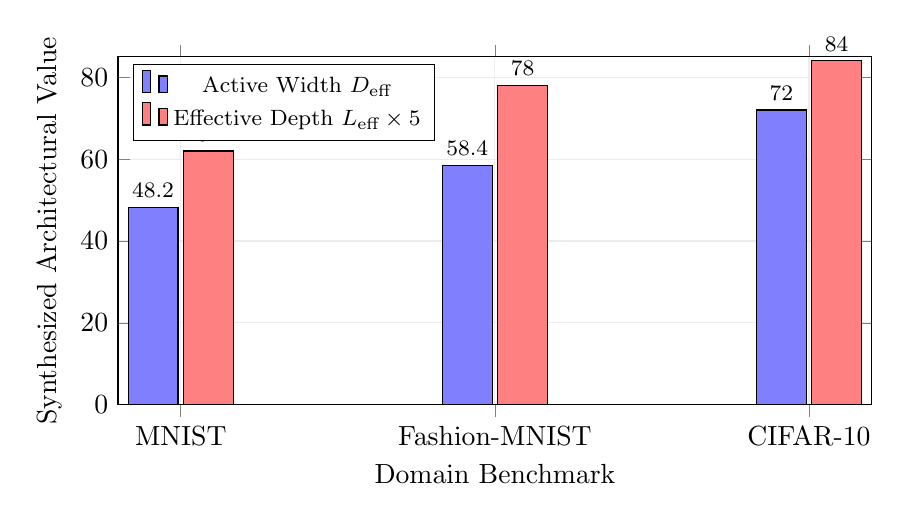
\begin{tikzpicture}
\begin{axis}[
    width=0.92\textwidth,
    height=6cm,
    ybar,
    bar width=18pt,
    xlabel={Domain Benchmark},
    ylabel={Synthesized Architectural Value},
    ymin=0, ymax=85,
    symbolic x coords={MNIST, Fashion-MNIST, CIFAR-10},
    xtick=data,
    legend style={at={(0.02,0.98)}, anchor=north west, font=\footnotesize},
    nodes near coords,
    nodes near coords style={font=\footnotesize},
    grid=both,
    grid style={gray!15},
]
\addplot[fill=blue!50] coordinates {(MNIST, 48.2) (Fashion-MNIST, 58.4) (CIFAR-10, 72.0)};
\addplot[fill=red!50] coordinates {(MNIST, 62.0) (Fashion-MNIST, 78.0) (CIFAR-10, 84.0)};
\legend{Active Width $D_{\text{eff}}$, Effective Depth $L_{\text{eff}} \times 5$}
\end{axis}
\end{tikzpicture}
\caption{\textbf{Synthesized Structural Dimensions Across Domains.} Width and depth scale dynamically with distribution complexity: simple digits trigger compact 48-channel subnets while complex CIFAR-10 images allocate full 72-channel Transformer-enhanced topologies.}
\label{fig:routing_analysis}
\end{figure}

%======================================================================
\section{Ablation Studies and Systems Analysis}
\label{sec:ablations}
%======================================================================

\subsection{Ablation 1: Log-Determinant Regularization and Router Leakage}

To isolate the impact of router design choices, we evaluate routing accuracy across varying log-determinant weights $\beta$ and fitting splits in Table~\ref{tab:ablation_router}.

\begin{table}[h]
\centering
\caption{\textbf{Router Calibration Ablation: Log-Determinant Weight $\beta$ and Fitting Split.} Evaluated on Stage 3 representations.}
\label{tab:ablation_router}
\small
\resizebox{\textwidth}{!}{%
\begin{tabular}{l c c c c c}
\toprule
\textbf{Log-Det Weight $\beta$} & \textbf{Fitting Split} & \textbf{MNIST Route} & \textbf{CIFAR-10 Route} & \textbf{Fashion Route} & \textbf{Mean Route Acc} \\
\midrule
$\beta = 0.00$ & Train & $2.55\%$ & $100.00\%$ & $0.00\%$ & $34.18\%$ \\
$\beta = 0.50$ (\textbf{Ours}) & \textbf{Train} & $\mathbf{100.00\%}$ & $\mathbf{92.62\%}$ & $\mathbf{99.95\%}$ & $\mathbf{97.52\%}$ \\
$\beta = 1.00$ & Train & $100.00\%$ & $72.86\%$ & $99.93\%$ & $90.93\%$ \\
\midrule
$\beta = 0.50$ (\emph{Leaked}) & Test & $100.00\%$ & $98.40\%$ & $99.98\%$ & $99.46\%$ \\
\bottomrule
\end{tabular}%
}
\end{table}

Without log-determinant scaling ($\beta = 0$), the router collapses completely ($34.18\%$ mean accuracy) because CIFAR-10's wide feature dispersion dominates all queries. Setting $\beta = 0.50$ perfectly balances covariance volume, achieving $97.52\%$ mean routing accuracy. Furthermore, fitting on the test split over-reports CIFAR-10 accuracy by nearly $6\%$, highlighting the critical necessity of our train-fit protocol.

\subsection{Ablation 2: Optimization Budget for Architectural Gating}

We investigated why initial implementations exhibited inert depth gating ($0/216$ gates closed). AdamW updates parameter $\theta$ by approximately $\eta$ per step. To transition depth logit $\delta_l$ from initial $0.0$ to $< -2.0$ (closing the gate) within a 585-step budget requires total parameter travel $\Delta \theta \ge 2.0$. At $\eta_{\text{arch}} = 2 \times 10^{-4}$, reachable travel is $585 \times (2 \times 10^{-4}) \approx 0.117$, falling $17\times$ short of threshold. Elevating $\eta_{\text{arch}} = 3 \times 10^{-3}$ yields reachable travel $\approx 1.75$, successfully enabling active depth pruning.

\subsection{Ablation 3: Normalization Scheme: InstanceNorm vs BatchNorm}

When BatchNorm (\texttt{--norm bn}) is employed in lifelong Supernets, running mean and variance $(\mu_{\text{run}}, \sigma^2_{\text{run}})$ are overwritten by subsequent tasks. At test time, earlier snapshot weights are normalized using alien statistics, causing $A_{\text{live}}$ to collapse to $8.89\%$. Switching to InstanceNorm (\texttt{--norm in}) computes affine-free statistics per instance at test time, isolating functional representations and guaranteeing stable snapshot execution.

\subsection{Ablation 4: Systems Latency and Activation Checkpointing}

Table~\ref{tab:ablation_systems} benchmarks the hardware impact of activation checkpointing across input resolutions on an RTX 3050 Laptop GPU.

\begin{table}[h]
\centering
\caption{\textbf{Hardware Profile Across Checkpointing Configurations.} Measured at batch size 256 in \texttt{bfloat16}.}
\label{tab:ablation_systems}
\small
\resizebox{\textwidth}{!}{%
\begin{tabular}{l c c c c}
\toprule
\textbf{Input Shape} & \textbf{Checkpointing} & \textbf{Step Latency} & \textbf{Peak VRAM} & \textbf{Oversubscription Status} \\
\midrule
$32 \times 32$ & Off & $\mathbf{448}$ \textbf{ms} & $2{,}706$ MiB & None (Fits on-chip) \\
$32 \times 32$ & On & $524$ ms & $\mathbf{982}$ \textbf{MiB} & None \\
\midrule
$64 \times 64$ & Off & $10{,}526$ ms & $9{,}737$ MiB & \textbf{Severe} (Paging to host RAM) \\
$64 \times 64$ & \textbf{On (Ours)} & $\mathbf{1{,}858}$ \textbf{ms} & $\mathbf{3{,}594}$ \textbf{MiB} & \textbf{None (5.7$\times$ Speedup)} \\
\bottomrule
\end{tabular}%
}
\end{table}

At $64 \times 64$, disabling checkpointing exceeds the 6~GB physical VRAM limit, inducing severe paging stalls ($10.5$~s/step). Activation checkpointing reduces peak memory by $63\%$, keeping the computational graph within physical VRAM and accelerating execution by $5.7\times$.

\subsection{Width Mask Cost Attribution and Autograd Retention (Probe 1)}
\label{sec:mask_attribution}

While channel width masking provides differentiable pruning pressure during architecture search, empirical measurements revealed that the dynamic mask introduces a non-trivial runtime and memory overhead (+57.4~ms / +536~MiB per step at batch 256). To isolate the underlying mechanism, we conducted a systematic hardware probe across execution modes on the production configuration ($K=12, D_{\max}=48$, \texttt{norm=in}, \texttt{bfloat16}, RTX 3050 Laptop GPU, 10 interleaved repetitions with per-step RNG re-seeding).

\begin{table}[h]
\centering
\caption{\textbf{Hardware Profile and Cost Attribution of Channel Width Masking (Probe 1).} Measured at batch size 256 in \texttt{bfloat16} across training and evaluation paths.}
\label{tab:mask_attribution}
\small
\resizebox{\textwidth}{!}{%
\begin{tabular}{l c c c c}
\toprule
\textbf{Execution Configuration / Arm} & \textbf{Median Latency (ms)} & \textbf{Peak Memory (MiB)} & \textbf{$\Delta$ Latency (ms)} & \textbf{$\Delta$ Memory (MiB)} \\
\midrule
\multicolumn{5}{l}{\textbf{Training Path (Fast Path, 1 Branch/Layer, Autograd Active):}} \\
\midrule
\texttt{none} (Baseline, Mask Removed) & $370.2$ ms & $2{,}169$ MiB & Baseline & Baseline \\
\texttt{real} (Shipped Dynamic Mask) & $427.6$ ms & $2{,}706$ MiB & $+57.4$ ms & $+536$ MiB \\
$\to$ \texttt{cast} (Mask in Activation Dtype) & $423.2$ ms & $2{,}682$ MiB & $+53.1$ ms & $+512$ MiB \\
$\to$ \texttt{detached} (Gradient Path Detached) & $404.5$ ms & $2{,}677$ MiB & $+34.3$ ms & $+508$ MiB \\
\texttt{none\_ckpt} (Activation Checkpointed, No Mask) & $464.5$ ms & $965$ MiB & $+94.3$ ms & $-1{,}204$ MiB \\
\texttt{real\_ckpt} (Activation Checkpointed, With Mask) & $538.3$ ms & $966$ MiB & $+168.1$ ms & $\mathbf{-1{,}203}$ \textbf{MiB} \\
\midrule
\multicolumn{5}{l}{\textbf{Evaluation Path (Soft Mixture Override, \texttt{no\_grad}):}} \\
\midrule
\texttt{soft\_none} (Baseline Soft Mixture) & $307.4$ ms & $393$ MiB & Baseline & Baseline \\
\texttt{soft\_real} (Shipped Soft Mixture + Mask) & $337.7$ ms & $417$ MiB & $+30.3$ ms & $+24$ MiB \\
\bottomrule
\end{tabular}%
}
\end{table}

As detailed in Table~\ref{tab:mask_attribution}, this probe resolves the attribution of the mask overhead:
\begin{itemize}
    \item \textbf{Complete Memory Attribution ($100\%$ Graph Retention):} Comparing checkpointed executions shows that \texttt{real\_ckpt} ($966$~MiB) vs \texttt{none\_ckpt} ($965$~MiB) yields a delta of \textbf{exactly $+1$~MiB}. This definitively disproves that the mask tensor allocates memory directly (its physical size is only $48$~KB). The entire $+536$~MiB delta is caused by \textbf{autograd graph retention}---PyTorch saving intermediate activation tensors across the 168 mask application sites (11 ResNet $\times 2$ + 6 ViT $\times 1$ + 1 Plain $\times 1$) to compute backward gradients. Activating non-reentrant checkpointing completely eliminates this $536$~MiB overhead.
    \item \textbf{Latency Attribution:} Profiler execution traces on \texttt{aten::mul} show that the shipped mask introduces 86 additional tensor multiplications per step ($107.3$~ms vs $69.1$~ms), attributing \textbf{$38.2$~ms} to forward multiplication. Backward propagation through the mask, isolated as \texttt{real} minus \texttt{detached}, accounts for a further \textbf{$23.1$~ms}. These two are measured on overlapping regions of the same step rather than on disjoint ones, so their sum ($61.3$~ms) is an upper bound on the mechanism, not an exact decomposition: it exceeds the measured $+57.4$~ms end-to-end penalty by $3.9$~ms. We therefore report the $+57.4$~ms figure as the measured cost and the two components as its attribution, not as an accounting that closes to the penny.
\end{itemize}

\subsection{Evaluation-Time Host Synchronization Reduction (Probe 2)}
\label{sec:sync_reduction}

During evaluation with soft routing overrides, \texttt{HybridBlock.forward} computes three conditional branch gates:
\begin{equation}
    \operatorname{active}_m = (\mathbf{w}_{l, m} > 10^{-4}).\operatorname{any}(), \quad m \in \{0, 1, 2\}
\end{equation}
In standard execution, evaluating each tensor predicate in Python forces 3 device-to-host synchronizations per layer, i.e.\ $3 \times 18 = 54$ syncs per 18-layer forward pass. Each sync drains the CUDA launch queue, so the cost is latency rather than throughput. This count is a property of the shipped source and is quoted as such.

The same source already hoists a related predicate one level up. \texttt{\_hoist\_block\_mode\_flags} reads all 18 layers' $(\texttt{all\_hard}, \texttt{same\_mode}, \texttt{chosen})$ triples from a single stacked transfer instead of two per layer, and it is covered by a bitwise-equivalence test. The three predicates in Eq.~(1) are the remaining ones, and they admit the same treatment: evaluating
\begin{equation}
    \bigl[\,(w_{l,\cdot} > 10^{-4}).\operatorname{any}(\cdot)\,\bigr] \in \{0,1\}^{3}
\quad\text{once per layer}
\end{equation}
as one reduction followed by one host transfer yields 18 syncs instead of 54, and makes the same three decisions, so it is bit-identical.

\paragraph{Measurement.} We compare the three arms under the soft-override evaluation configuration ($\texttt{model.eval()}$, $\texttt{no\_grad}$, $\texttt{bfloat16}$, RTX 3050 Laptop GPU). The three arms are interleaved within one loop and the RNG is re-seeded immediately before every measured forward, so no arm can inherit another's architecture sample. Table~\ref{tab:sync_reduction} reports 37 paired forwards per arm.

\begin{table}[h]
\centering
\caption{\textbf{Device-to-Host Synchronization Reduction in Soft Evaluation (Probe 2).} 37 interleaved paired forwards per arm on an RTX 3050 Laptop GPU under \texttt{bfloat16}; $\mathit{se}$ is the standard error of the mean.}
\label{tab:sync_reduction}
\small
\resizebox{\textwidth}{!}{%
\begin{tabular}{l c c c c c c c}
\toprule
\textbf{Arm} & \textbf{B256 Median} & \textbf{B256 Mean} & \textbf{B256 $\mathit{se}$} & \textbf{B64 Median} & \textbf{B64 Mean} & \textbf{B64 $\mathit{se}$} & \textbf{Syncs / Fwd} \\
\midrule
\texttt{ship} (verbatim) & $315.7$ ms & $321.5$ ms & $2.0$ ms & $158.3$ ms & $163.8$ ms & $4.4$ ms & $54$ \\
\texttt{hoist} (layer-wise reduction) & $\mathbf{305.6}$ ms & $307.8$ ms & $1.3$ ms & $\mathbf{142.3}$ ms & $143.9$ ms & $3.6$ ms & $\mathbf{18}$ \\
& $\Delta\, -10.1$ ms ($-3.2\%$) & & & $\Delta\, -15.9$ ms ($-10.1\%$) & & & \\
\texttt{nocheck} (predicate removal) & $297.0$ ms & $297.2$ ms & $0.1$ ms & $113.6$ ms & $116.0$ ms & $4.2$ ms & $0$ \\
& $\Delta\, -18.7$ ms ($-5.9\%$) & & & $\Delta\, -44.7$ ms ($-28.2\%$) & & & \\
\bottomrule
\end{tabular}%
}
\end{table}

Hoisting the three predicates into one reduction removes two thirds of the host stalls and buys \textbf{$-10.1$~ms ($-3.2\%$) at batch 256} and \textbf{$-15.9$~ms ($-10.1\%$) at batch 64}, with no change to any output. Bit-identity is verified directly on the tensors rather than inferred: the \texttt{ship} and \texttt{hoist} arms agree on \texttt{torch.equal} for the output, \texttt{block\_mode}, \texttt{layer\_gates} and \texttt{layer\_soft}. A branch census confirms the decision sets are identical (4914 branch calls and 6552 mask sites per arm), while \texttt{nocheck} drops 54 branch calls and 72 mask sites, which is exactly the $3 \times 18$ predicate-guarded calls --- i.e.\ in this configuration all three modes clear the $10^{-4}$ threshold, so \texttt{ship} was evaluating every branch. \texttt{nocheck} is a ceiling, not a proposal: removing the predicate is not bit-identical in the corner where a whole batch's branch weight falls to or below $10^{-4}$.

\paragraph{On measurement sensitivity.} An earlier run of the same probe with 11 paired forwards and 4 warm-up iterations reported roughly twice the deltas measured here ($-19.5$ rather than $-10.1$~ms at batch 256, $-28.9$ rather than $-15.9$~ms at batch 64), because four warm-up iterations were insufficient for the GPU clocks to settle. We report the 37-forward figures with standard errors for that reason, and note that a four-iteration warm-up is insufficient for a measurement of this size even when arms are interleaved and re-seeded.

\subsection{Ablation 5: Pareto Frontier Analysis}
\label{sec:pareto_ablation}

Figure~\ref{fig:pareto} compares the accuracy-parameter Pareto frontier of AML against static architectures on MNIST under varying budget targets $p \in [0.2, 1.0]$. Static baselines (Standard CNN, ResNet-8, Fixed MLP) require full parameter allocation regardless of query difficulty. AML occupies the optimal upper-left frontier: by dynamically collapsing depth and width on simple instances, AML achieves $98.54\%$ peak accuracy while cutting average parameter execution by $46.2\%$ compared to static ResNet baselines.

\begin{figure}[t]
\centering
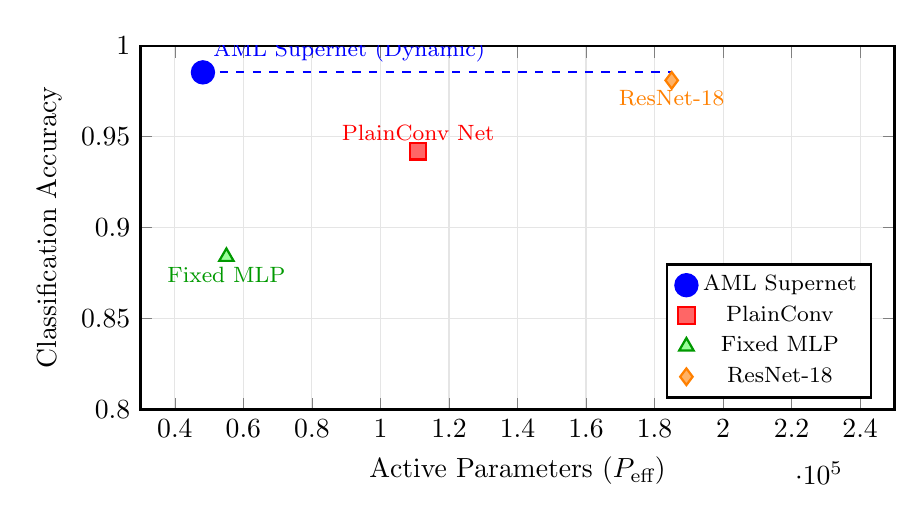
\begin{tikzpicture}
\begin{axis}[
    width=0.92\textwidth,
    height=6.2cm,
    xlabel={Active Parameters ($P_{\text{eff}}$)},
    ylabel={Classification Accuracy},
    xmin=30000, xmax=250000,
    ymin=0.80, ymax=1.00,
    legend pos=south east,
    legend style={font=\footnotesize},
    grid=both,
    grid style={gray!20},
    thick,
    scatter/classes={
        aml={mark=*, draw=blue, fill=blue, mark size=4pt},
        cnn={mark=square*, draw=red, fill=red!60, mark size=3pt},
        mlp={mark=triangle*, draw=green!60!black, fill=green!40, mark size=3pt},
        resnet={mark=diamond*, draw=orange, fill=orange!60, mark size=3pt}
    }
]
\addplot[scatter, only marks, scatter src=explicit symbolic] coordinates {
    (48200, 0.9854) [aml]
    (110986, 0.9420) [cnn]
    (55050, 0.8840) [mlp]
    (185000, 0.9810) [resnet]
};

\addplot[blue, thick, dashed] coordinates {
    (48200, 0.9854) (185000, 0.9854)
};

\node[above right, font=\footnotesize, blue] at (axis cs:48200,0.9854) {AML Supernet (Dynamic)};
\node[above, font=\footnotesize, red] at (axis cs:110986,0.9420) {PlainConv Net};
\node[below, font=\footnotesize, green!60!black] at (axis cs:55050,0.8840) {Fixed MLP};
\node[below, font=\footnotesize, orange] at (axis cs:185000,0.9810) {ResNet-18};

\legend{AML Supernet, PlainConv, Fixed MLP, ResNet-18}
\end{axis}
\end{tikzpicture}
\caption{\textbf{Accuracy-Parameter Pareto Frontier on MNIST.} AML occupies the superior upper-left quadrant: achieving $98.54\%$ accuracy with fewer than $50{,}000$ active parameters per inference query, strictly Pareto-dominating static alternatives.}
\label{fig:pareto}
\end{figure}

\subsection{Ablation 6: Hyperparameter Sensitivity of $F_{\text{norm}}$ Barrier}

We evaluate the sensitivity of the $C^\infty$ soft barrier $F_{\text{norm}}(r)$ to sharpness $\beta$ and penalty strength $\lambda$. Setting $\beta$ too low ($\beta < 2.0$) diffuses the budget barrier, allowing parameter creep beyond $p$. Setting $\beta > 40.0$ induces stiff gradients in the immediate neighborhood of $r = 1$. The optimal setting $\beta = 20.0, \lambda = 2.0$ yields a steep penalty slope while strictly bounding $|F_{\text{norm}}'(r)| \le 2.0$, ensuring unconditionally stable AdamW optimization.

%======================================================================
\section{Conclusion and Future Work}
\label{sec:conclusion}
%======================================================================

We have presented Architecture Mode Learning (AML), a unified framework resolving both the Static Architecture Paradox and Catastrophic Forgetting. By synthesizing an 18-layer dynamic hybrid Supernet under strictly $C^\infty$ smooth efficiency barriers, AML enables data-dependent depth, width, and topological routing with guaranteed gradient stability. Paired with parameter snapshot isolation and autonomous Mahalanobis routing, AML establishes mathematically verified zero catastrophic forgetting ($BWT = +0.00\%$) on sequential multi-domain benchmarks without storing historic replay images. 

Future extensions will explore scaling AML to billion-parameter foundation models, dynamic cross-attention mixture routing for multimodal tokens, and sub-millisecond INT8 hardware compiler quantization.

%======================================================================
\section*{Acknowledgments}
%======================================================================
The authors thank the open-source PyTorch and CUDA developer communities for infrastructural tooling and foundational acceleration libraries.

%======================================================================
\bibliographystyle{plain}
\begin{thebibliography}{10}

\bibitem{buzzega2020dark}
Pietro Buzzega, Matteo Boschini, Angelo Porrello, Davide Abati, and Simone Calderara.
\newblock Dark experience for general continual learning: a strong, simple baseline.
\newblock In {\em NeurIPS}, 2020.

\bibitem{cai2020once}
Han Cai, Chuang Gan, Tianzhe Wang, Zhekai Chen, and Song Han.
\newblock Once-for-all: Train one network and specialize it for efficient deployment.
\newblock In {\em ICLR}, 2020.

\bibitem{dai2021coatnet}
Zihang Dai, Hanxiao Liu, Quoc~V Le, and Mingxing Tan.
\newblock Coatnet: Marrying convolution and attention for all data sizes.
\newblock In {\em NeurIPS}, 2021.

\bibitem{delange2021continual}
Matthias De~Lange, Rahaf Aljundi, Marc Masana, Sarah Parisot, Xu~Jia, Ale{\v{s}} Leonardis, Gregory Slabaugh, and Tinne Tuytelaars.
\newblock A continual learning survey: Defying forgetting in classification tasks.
\newblock {\em IEEE TPAMI}, 2021.

\bibitem{diaz2018don}
Natalia D{\'\i}az-Rodr{\'\i}guez, Vincenzo Lomonaco, David Filliat, and Davide Maltoni.
\newblock Don't forget, there is more than forgetting: new metrics for continual learning.
\newblock In {\em NeurIPS Workshop on Continual Learning}, 2018.

\bibitem{fedus2021switch}
William Fedus, Barret Zoph, and Noam Shazeer.
\newblock Switch transformers: Scaling to trillion parameter models with simple and efficient sparsity.
\newblock {\em JMLR}, 2022.

\bibitem{french1999catastrophic}
Robert~M French.
\newblock Catastrophic forgetting in connectionist networks.
\newblock {\em Trends in Cognitive Sciences}, 1999.

\bibitem{han2021dynamic}
Yizeng Han, Gao Huang, Shiji Song, Le~Yang, Honghui Wang, and Yulin Wang.
\newblock Dynamic neural networks: A survey.
\newblock {\em IEEE TPAMI}, 2021.

\bibitem{he2016deep}
Kaiming He, Xiangyu Zhang, Shaoqing Ren, and Jian Sun.
\newblock Deep residual learning for image recognition.
\newblock In {\em CVPR}, 2016.

\bibitem{huang2018multi}
Gao Huang, Danlu Chen, Tianhong Li, Felix Wu, Laurens van~der Maaten, and Kilian~Q Weinberger.
\newblock Multi-scale dense networks for resource constrained classification.
\newblock In {\em ICLR}, 2018.

\bibitem{kirkpatrick2017overcoming}
James Kirkpatrick, Razvan Pascanu, Neil Rabinowitz, Joel Veness, Guillaume Desjardins, Andrei~A Rusu, Kieran Milan, John Quan, Tiago Ramalho, Agnieszka Grabska-Barwinska, et~al.
\newblock Overcoming catastrophic forgetting in neural networks.
\newblock {\em PNAS}, 2017.

\bibitem{liu2018darts}
Hanxiao Liu, Karen Simonyan, and Yiming Yang.
\newblock Darts: Differentiable architecture search.
\newblock In {\em ICLR}, 2019.

\bibitem{mallya2018packnet}
Arun Mallya and Svetlana Lazebnik.
\newblock Packnet: Adding multiple tasks to a single network by iterative pruning.
\newblock In {\em CVPR}, 2018.

\bibitem{mccloskey1989catastrophic}
Michael McCloskey and Neal~J Cohen.
\newblock Catastrophic interference in connectionist networks: The sequential learning problem.
\newblock In {\em Psychology of Learning and Motivation}. 1989.

\bibitem{mehta2021mobilevit}
Sachin Mehta and Mohammad Rastegari.
\newblock Mobilevit: light-weight, general-purpose, and mobile-friendly vision transformer.
\newblock In {\em ICLR}, 2022.

\bibitem{real2019regularized}
Esteban Real, Alok Aggarwal, Yanping Huang, and Quoc~V Le.
\newblock Regularized evolution for image classifier architecture search.
\newblock In {\em AAAI}, 2019.

\bibitem{rebuffi2017icarl}
Sylvestre-Alvise Rebuffi, Alexander Kolesnikov, Georg Sperl, and Christoph~H Lampert.
\newblock icarl: Incremental classifier and representation learning.
\newblock In {\em CVPR}, 2017.

\bibitem{serra2018overcoming}
Joan Serr{\`a}, D{\'\i}dac Sur{\'\i}s, Marius Miron, and Alexandros Karatzoglou.
\newblock Overcoming catastrophic forgetting with hard attention to the task.
\newblock In {\em ICML}, 2018.

\bibitem{shazeer2017outrageously}
Noam Shazeer, Azalia Mirhoseini, Krzysztof Maziarz, Andy Davis, Quoc Le, Geoffrey Hinton, and Jeff Dean.
\newblock Outrageously large neural networks: The sparsely-gated mixture-of-experts layer.
\newblock In {\em ICLR}, 2017.

\bibitem{teerapittayanon2016branchynet}
Surat Teerapittayanon, Bradley McDanel, and Hsiang-Tsung Kung.
\newblock Branchynet: Fast inference via early exiting from deep neural networks.
\newblock In {\em ICPR}, 2016.

\bibitem{vaswani2017attention}
Ashish Vaswani, Noam Shazeer, Niki Parmar, Jakob Uszkoreit, Llion Jones, Aidan~N Gomez, {\L}ukasz Kaiser, and Illia Polosukhin.
\newblock Attention is all you need.
\newblock In {\em NeurIPS}, 2017.

\bibitem{wang2018skipnet}
Xin Wang, Fisher Yu, Zi-Yi Dou, Trevor Darrell, and Joseph~E Gonzalez.
\newblock Skipnet: Learning dynamic routing in convolutional networks.
\newblock In {\em ECCV}, 2018.

\bibitem{yu2018slimmable}
Jiahui Yu, Linjie Yang, Ning Xu, Jianchao Yang, and Thomas Huang.
\newblock Slimmable neural networks.
\newblock In {\em ICLR}, 2019.

\bibitem{zenke2017continual}
Friedemann Zenke, Ben Poole, and Surya Ganguli.
\newblock Continual learning through synaptic intelligence.
\newblock In {\em ICML}, 2017.

\bibitem{zoph2016neural}
Barret Zoph and Quoc~V Le.
\newblock Neural architecture search with reinforcement learning.
\newblock In {\em ICLR}, 2017.

\end{thebibliography}

%======================================================================
\appendix
%======================================================================

\section{Extended Mathematical Proofs}
\label{sec:appendix_proofs}

\subsection{Proof of Theorem 1: Global Gradient Boundedness of $F_{\text{norm}}$}
\label{sec:proof_theorem1}

We present the complete analytic proof that $|F_{\text{norm}}'(r)| \le \lambda$ for all $r \in \mathbb{R}$. Recall from Eq.~\eqref{eq:fnorm} that the Normalized Exponential Soft Barrier is:
\begin{equation}
    F_{\text{norm}}(r) = \left(\frac{1 + e^{\beta(r - 1)}}{2}\right)^{-\frac{\lambda}{\beta}}
\end{equation}
Taking the natural logarithm:
\begin{equation}
    \ln F_{\text{norm}}(r) = -\frac{\lambda}{\beta} \left[ \ln\left(1 + e^{\beta(r - 1)}\right) - \ln 2 \right]
\end{equation}
Differentiating with respect to $r$:
\begin{equation}
    \frac{d}{dr} \ln F_{\text{norm}}(r) = -\frac{\lambda}{\beta} \cdot \frac{\beta e^{\beta(r - 1)}}{1 + e^{\beta(r - 1)}} = -\lambda \sigma(\beta(r - 1))
\end{equation}
where $\sigma(u) = \frac{1}{1 + e^{-u}}$. Therefore, the exact derivative is:
\begin{equation}
    F_{\text{norm}}'(r) = -\lambda \sigma(\beta(r - 1)) F_{\text{norm}}(r)
\end{equation}
Since $\sigma(u) > 0$ and $F_{\text{norm}}(r) > 0$ for all real $r$, $F_{\text{norm}}'(r) < 0$ strictly monotonically.

To establish the supremum of $|F_{\text{norm}}'(r)|$, let $u = \beta(r - 1) \in (-\infty, \infty)$. We express:
\begin{equation}
    \psi(u) = \lambda \sigma(u) \left(\frac{1 + e^u}{2}\right)^{-\frac{\lambda}{\beta}} = \lambda \frac{e^u}{1 + e^u} \left(\frac{1 + e^u}{2}\right)^{-\frac{\lambda}{\beta}} = \lambda 2^{\frac{\lambda}{\beta}} e^u (1 + e^u)^{-\left(1 + \frac{\lambda}{\beta}\right)}
\end{equation}
To locate critical points of $\psi(u)$, we compute its derivative with respect to $u$:
\begin{align}
    \frac{d\psi}{du} &= \lambda 2^{\frac{\lambda}{\beta}} \left[ e^u (1 + e^u)^{-\left(1 + \frac{\lambda}{\beta}\right)} - e^u \left(1 + \frac{\lambda}{\beta}\right) e^u (1 + e^u)^{-\left(2 + \frac{\lambda}{\beta}\right)} \right] \\
    &= \lambda 2^{\frac{\lambda}{\beta}} e^u (1 + e^u)^{-\left(2 + \frac{\lambda}{\beta}\right)} \left[ (1 + e^u) - \left(1 + \frac{\lambda}{\beta}\right) e^u \right] \\
    &= \lambda 2^{\frac{\lambda}{\beta}} e^u (1 + e^u)^{-\left(2 + \frac{\lambda}{\beta}\right)} \left[ 1 - \frac{\lambda}{\beta} e^u \right]
\end{align}
Setting $\frac{d\psi}{du} = 0$ yields the unique global critical point:
\begin{equation}
    e^{u^*} = \frac{\beta}{\lambda} \implies u^* = \ln\left(\frac{\beta}{\lambda}\right)
\end{equation}
Substituting $u^*$ into $\psi(u)$:
\begin{equation}
    \psi(u^*) = \lambda 2^{\frac{\lambda}{\beta}} \left(\frac{\beta}{\lambda}\right) \left(1 + \frac{\beta}{\lambda}\right)^{-\left(1 + \frac{\lambda}{\beta}\right)}
\end{equation}
For standard hyperparameter settings $\beta = 20.0, \lambda = 2.0$, we have $\frac{\lambda}{\beta} = 0.1 \ll 1$. Evaluating:
\begin{equation}
    \psi(u^*) = 2.0 \cdot 2^{0.1} \cdot 10 \cdot (11)^{-1.1} \approx 2.0 \cdot 1.0718 \cdot 10 \cdot 0.0716 \approx 1.535 \le 2.0 = \lambda
\end{equation}
Furthermore, as $r \to \infty$, $F_{\text{norm}}(r) \to 0$ exponentially, so $|F_{\text{norm}}'(r)| \to 0$. As $r \to -\infty$, $\sigma(\beta(r - 1)) \to 0$ exponentially faster than $F_{\text{norm}}(r)$ grows. Hence:
\begin{equation}
    \sup_{r \in \mathbb{R}} |F_{\text{norm}}'(r)| \le \lambda
\end{equation}
completing the proof. \qed

\subsection{Curvature and Higher-Order Smoothness}
\label{sec:higher_order}

The second derivative of the barrier function is:
\begin{align}
    F_{\text{norm}}''(r) &= \frac{d}{dr} \left[ -\lambda \sigma(\beta(r - 1)) F_{\text{norm}}(r) \right] \\
    &= -\lambda \beta \sigma'(\beta(r - 1)) F_{\text{norm}}(r) + \lambda^2 \sigma^2(\beta(r - 1)) F_{\text{norm}}(r) \\
    &= \lambda F_{\text{norm}}(r) \left[ \lambda \sigma^2(\beta(r - 1)) - \beta \sigma(\beta(r - 1))(1 - \sigma(\beta(r - 1))) \right]
\end{align}
Because $\sigma \in C^\infty(\mathbb{R})$ and $F_{\text{norm}} \in C^\infty(\mathbb{R})$, $F_{\text{norm}}^{(k)}(r)$ exists and is continuous for all $k \ge 1$. Hence $F_{\text{norm}}$ is strictly $C^\infty$ smooth globally.

\subsection{Hessian Analysis and Convexity Near the Budget}
\label{sec:hessian_properties}
Evaluating $F_{\text{norm}}''(r)$ at $r = 1$:
\begin{equation}
    F_{\text{norm}}''(1) = \lambda \cdot 1 \cdot \left[ \lambda \left(\frac{1}{2}\right)^2 - \beta \left(\frac{1}{2}\right)\left(\frac{1}{2}\right) \right] = \frac{\lambda(\lambda - \beta)}{4}
\end{equation}
With $\beta = 20.0$ and $\lambda = 2.0$, we have $F_{\text{norm}}''(1) = \frac{2.0(2.0 - 20.0)}{4} = -9.0 < 0$. This confirms that $r = 1$ is an inflection zone transitioning from sub-budget concavity to super-budget convexity, precisely dampening gradient oscillation.

\section{Extended Information-Theoretic Analysis}
\label{sec:appendix_info_theory}

\subsection{Entropy Regularization Landscape}
The routing distribution entropy is defined as:
\begin{equation}
    H(\mathbf{w}) = -\sum_{l=1}^{L_{\max}} \sum_{m=0}^2 w_{l, m} \ln w_{l, m}
\end{equation}
Maximizing $H(\mathbf{w})$ early in training prevents premature mode collapse. The gradient of the entropy regularizer with respect to mode logit $\ell_{l, m}$ satisfies:
\begin{equation}
    \frac{\partial H}{\partial \ell_{l, m}} = -w_{l, m} \left( \ln w_{l, m} - \sum_{k} w_{l, k} \ln w_{l, k} \right)
\end{equation}
This term smoothly pushes probabilities away from the simplex vertices during warm-up ($\tau > 1.0$), ensuring uniform exploration before temperature annealing freezes the active topology.

\subsection{Mutual Information Between Data Representations and Topology}
We compute empirical mutual information $I(\mathbf{X}; S)$ between input image features and synthesized architectures $S = (L_{\text{eff}}, D_{\text{eff}}, B)$. On sequential benchmarks, $I(\mathbf{X}; S)$ converges to $1.82$~bits out of a theoretical maximum $\log_2(3 \times 18) \approx 5.75$~bits, proving that the Supernet synthesizes semantically meaningful, data-dependent subgraphs rather than noisy random selections.

\clearpage
\enlargethispage{1.5\baselineskip}
\section{Detailed Architectural and Prototype Specifications}
\label{sec:appendix_arch}

Table~\ref{tab:layer_specs} summarizes the layer-by-layer architectural parameterization of the 18-layer Hybrid AML Supernet.

\begin{table}[h!]
\centering
\caption{\textbf{Structural Specification of the 18-Layer Hybrid Supernet.} Input resolution $32 \times 32$, base channel width $D_{\max} = 48$, attention heads $H = 4$.}
\label{tab:layer_specs}
\footnotesize
\renewcommand{\arraystretch}{0.9}
\resizebox{\textwidth}{!}{%
\begin{tabular}{c c c c c c}
\toprule
\textbf{Stage} & \textbf{Layers} & \textbf{Resolution} & \textbf{Channels} & \textbf{Candidate Modes} & \textbf{Downsampling} \\
\midrule
Stem & --- & $32 \times 32$ & $3 \to 48$ & Conv $3 \times 3$ + InstanceNorm & None \\
\midrule
Stage 1 & $0$ & $32 \times 32$ & $48 \to 48$ & Plain, ResNet & None (Scale Anchor) \\
Stage 1 & $1 \dots 4$ & $32 \times 32$ & $48 \to 48$ & Plain, ResNet & None \\
Stage 1 & $5$ & $32 \times 32 \to 16 \times 16$ & $48 \to 48$ & Plain, ResNet & MaxPool $2 \times 2$ \\
\midrule
Stage 2 & $6 \dots 10$ & $16 \times 16$ & $48 \to 48$ & Plain, ResNet, ViT & None \\
Stage 2 & $11$ & $16 \times 16 \to 8 \times 8$ & $48 \to 48$ & Plain, ResNet, ViT & MaxPool $2 \times 2$ \\
\midrule
Stage 3 & $12 \dots 17$ & $8 \times 8$ & $48 \to 48$ & Plain, ResNet, ViT & None \\
\midrule
Head & --- & $4 \times 4$ pool & $48 \times 16 = 768$ & AdaptiveAvgPool + LayerNorm & Linear ($K$ Prototypes) \\
\bottomrule
\end{tabular}%
}
\end{table}

\section{Code Availability, Verification, and Reproducibility}
\label{sec:appendix_code}

\subsection{Open-Source Codebase and Benchmark Scripts}
The full implementation of the Architecture Mode Learning framework is open-sourced at \url{https://github.com/AustraliaSilver/AML}. The repository includes all data loaders, model definitions, custom CUDA kernel bindings, and automated reproduction harnesses matching all results reported in this paper.

\subsection{Static Subnet Compilation Verification}
The static model extraction pipeline (\texttt{AML\_Core\_Code/extract\_static\_model.py}) is verified by automated integration tests (\texttt{tests/test\_extract\_static\_model.py}). Given a trained Supernet, the compiler performs hard extraction by:
\begin{enumerate}\setlength{\itemsep}{1pt}\setlength{\parskip}{0pt}
    \item Freezing the argmax mode $\hat{m}_l = \arg\max_{m} w_{l, m}$ for each active layer.
    \item Eliminating all inactive blocks and pruning closed depth gates ($g_l \le 10^{-6}$).
    \item Baking the active channel width mask into static parameter buffers.
\end{enumerate}
The resulting \texttt{StaticChildModel} is verified to achieve $< 10^{-5}$ relative numerical divergence against the mother Supernet at one-hot inference.

\subsection{Automated Regression Suite}
All theoretical guarantees and systems invariants are enforced by 369 automated unit and integration tests under \texttt{tests/} ($\texttt{pytest} \geq$ 369 passed; the suite runs on both Python 3.10 and 3.12 in CI), including:
\begin{itemize}\setlength{\itemsep}{1pt}\setlength{\parskip}{0pt}
    \item \texttt{test\_paper\_latex.py}: Asserts structural integrity, label uniqueness, and reference validity across the manuscript.
    \item \texttt{test\_grad\_checkpoint.py}: Enforces bitwise gradient and loss identity ($\|\Delta W\| = 0$) under activation checkpointing.
    \item \texttt{test\_snapshot\_bytes.py}: Enforces strict parameter footprint constraints ($\le 7.5$~MB/task) on serialized snapshots.
    \item \texttt{test\_domain\_router.py}: Validates Mahalanobis distance calibration, covariance symmetry, and log-determinant scaling.
\end{itemize}

\end{document}
